\documentclass[msc,twoside]{ppgccufmg}

\usepackage[brazil]{babel}
\usepackage[utf8]{inputenc}
\usepackage[T1]{fontenc}
\usepackage{type1ec}
\usepackage{graphicx}
\usepackage{multirow}
\usepackage{amsfonts}
\usepackage[cmex10]{amsmath}
\usepackage{subcaption}
\usepackage{caption}
\usepackage[a4paper,
  portuguese,
  bookmarks=true,
  bookmarksnumbered=true,
  linktocpage,
  colorlinks,
  citecolor=black,
  urlcolor=black,
  linkcolor=black,
  filecolor=black,
  ]{hyperref}
\usepackage[square]{natbib}
\usepackage{todonotes}
\usepackage{rotating}
\usepackage[chapter]{algorithm}
\usepackage{algorithmic}

% \makeatletter
% \renewcommand*{\ALG@name}{Algoritmo}
% \renewcommand{\ALG@name}{Algoritmo}
% \renewcommand{\listalgorithmname}{Lista de Algoritmos}
% \makeatother

\usepackage[toc, nonumberlist, sort=def]{glossaries}
\newglossary{acro}{acro}{sb2}{Lista de Acrônimos}
\newglossary{symb}{symb}{sb3}{Lista de Símbolos}
\newglossary{symbh}{symbh}{sb4}{Lista de Símbolos}

\makeglossaries

\begin{document}

\newcommand{\gl}[1]{\gls{#1}}
\newcommand{\sy}[1]{\glssymbol{#1}}
\newcommand{\de}[1]{\glsdesc{#1}}

\newcommand{\newacro}[3]{\newglossaryentry{#1}{type=acro,name={#2},description={#3}}}
\newcommand{\newsymb}[3]{\newglossaryentry{#1}{type=symb,symbol={#2},name={#2},description={#3}}}
\newcommand{\newsymbh}[3]{\newglossaryentry{#1}{type=symbh,symbol={#2},name={#2},description={#3}}}

\renewcommand{\listalgorithmname}{Lista de Algoritmos}

% Image Commands

\newcommand{\img}[2]{
  \includegraphics[width=#2]{img/#1}
}

% \imgosize{#1}{#2}
\newcommand{\fig}[3]{
\begin{figure}[htpb]
\centering
\setlength{\fboxsep}{0pt}
#2
\caption{#3}
\label{fig:#1}
\end{figure}
}

\newcommand{\specialcell}[2][c]{%
  \begin{tabular}[#1]{@{}c@{}}#2\end{tabular}}

\newcommand{\environment}{\ensuremath{\mathbb{R}^3}}

% Shortcut definitions

\newcommand{\set}[1]{\ensuremath{\boldsymbol{\mathcal{#1}}}}
\newcommand{\setitem}[2]{\ensuremath{#1_{#2}}}
\newcommand{\setlist}[3]{#1\ $=$\ \{\setitem{#2}{1}, \setitem{#2}{2}, ..., \setitem{#2}{#3}\}}
\newcommand{\setlistdef}[2]{\{\setitem{#1}{1}, \setitem{#1}{2}, ..., \setitem{#1}{#2}\}}

\newcommand{\robotset}{\set{R}} % conjunto de robôs
\newcommand{\robotsetqt}{\ensuremath{k}}
\newcommand{\robot}[1]{\setitem{r}{#1}}
\newcommand{\robotlist}{\setlist{\robotset}{r}{\robotsetqt}}
\newcommand{\robotlistdef}{\setlistdef{r}{\robotsetqt}}

\newcommand{\obstacleset}{\set{B}} % conjunto de obstáculos
\newcommand{\obstaclesetqt}{\ensuremath{x}}
\newcommand{\obstacle}[1]{\setitem{b}{#1}}
\newcommand{\obstaclelist}{\setlist{\obstacleset}{b}{\obstaclesetqt}}
\newcommand{\obstaclelistdef}{\setlistdef{b}{\obstaclesetqt}}

\newcommand{\objectset}{\set{O}} % conjunto de objetos
\newcommand{\objectsetqt}{\ensuremath{y}}
\newcommand{\object}[1]{\setitem{o}{#1}}
\newcommand{\objectlist}{\setlist{\objectset}{o}{\objectsetqt}}
\newcommand{\objectlistdef}{\setlistdef{o}{\objectsetqt}}

\newcommand{\workobjectset}{\set{W_O}}

\newcommand{\robotplanset}{\set{RP}} % conjunto de planos
\newcommand{\robotplansetqt}{\ensuremath{j}}
\newcommand{\robotplan}[1]{\setitem{rp}{#1}}
\newcommand{\robotplanlist}{\setlist{\robotplanset}{rp}{\robotplansetqt}}

% \newcommand{\executionplanset}{\set{EP}} % conjunto de planos
% \newcommand{\executionplansetqt}{\ensuremath{h}}
% \newcommand{\executionplan}[1]{\setitem{ep}{#1}}
% \newcommand{\executionplanlist}{\setlist{\executionplanset}{ep}{\executionplansetqt}}
% \newcommand{\executionplanname}{\emph{Execution Plan}}
% \newcommand{\executionplansetnotation}{\ensuremath{\executionplanset \subset \robotplanset}}

% \newcommand{\executionplanminset}{\ensuremath{\executionplanset{*}}} % conjunto com custo minimo de segmentos

\newcommand{\segmentset}{\set{S}} % conjunto de segmentos
\newcommand{\segmentsetqt}{\ensuremath{e}}
\newcommand{\segment}[1]{\setitem{s}{#1}}
\newcommand{\segmentlist}{\setlist{\segmentset}{s}{\segmentsetqt}}

\newcommand{\segmentpointset}{\ensuremath{\set{S}_p}} % conjunto de pontos de segmentação
\newcommand{\segmentpointsetqt}{\ensuremath{z}}
\newcommand{\segmentpoint}[1]{\setitem{sp}{#1}}
\newcommand{\segmentpointlist}{\setlist{\segmentpointset}{sp}{\segmentpointsetqt}}

\newcommand{\segmentpointfirst}[1]{\ensuremath{\segmentpoint{#1}^1}}
\newcommand{\segmentpointsecond}[1]{\ensuremath{\segmentpoint{#1}^2}}


\newcommand{\typeland}{ground}
\newcommand{\typeaerial}{aerial}
\newcommand{\typeset}{\set{T}} % conjunto de tipos de movimentação
\newcommand{\typelist}{\ensuremath{\typeset=\ \{}\typeland, \typeaerial\ensuremath{\}}}
\newcommand{\type}[1]{\setitem{t}{#1}}

% \newcommand{\plantypestart}{initial}
% \newcommand{\plantypetransition}{transition}
% \newcommand{\plantypemove}{movement}
% \newcommand{\plantypeset}{\set{TP}} % conjunto de tipos de plano
% \newcommand{\plantypelist}{\ensuremath{\plantypeset=\ \{}\plantypestart, \plantypetransition, \plantypemove\ensuremath{\}}}
% \newcommand{\plantype}[1]{\setitem{tp}{#1}}

\newcommand{\movementtypepremove}{preparação}
\newcommand{\movementtypemove}{transporte}
\newcommand{\movementtypeset}{\set{T_{M}}} % conjunto de tipos de plano
\newcommand{\movementtypelist}{\ensuremath{\movementtypeset=\{}\movementtypepremove, \movementtypemove\ensuremath{\}}}
\newcommand{\movementtype}[1]{\setitem{tm}{#1}}

\newcommand{\tokenset}{\set{TO}}
\newcommand{\tokensetqt}{\ensuremath{u}}
\newcommand{\tokeni}[1]{\setitem{to}{#1}}
\newcommand{\token}{\emph{token}}
\newcommand{\tokenlist}{\setlist{\tokenset}{to}{\tokensetqt}}

\newcommand{\workspace}{\ensuremath{\boldsymbol{\mathcal{W}}}} % àrea de trabalho
\newcommand{\wcell}{\ensuremath{\mathtt{c}}}
\newcommand{\wcelli}[1]{\ensuremath{\mathtt{c_#1}}}

\newcommand{\allocationgraph}{\ensuremath{\mathcal{AG}}}
\newcommand{\allocationgraphcompress}{\ensuremath{\mathcal{AG}_c}}

\newcommand{\robotinitialstate}{\ensuremath{I}}
\newcommand{\robotinitialstatei}[1]{\ensuremath{I_{#1}}}

\newcommand{\celldimension}{\ensuremath{d}}
\newcommand{\deslocationfactor}{\ensuremath{l}}

\newcommand{\movementset}{\set{M}}

\newcommand{\movementforward}{forward}
\newcommand{\movementbackward}{backward}
\newcommand{\movementleft}{left}
\newcommand{\movementright}{right}
\newcommand{\movementup}{up}
\newcommand{\movementdown}{down}

\newcommand{\movementslist}{\ensuremath{\movementset=\ \{\movementleft, \movementright, \movementforward, \movementbackward, \movementup, \movementdown\}}}
\newcommand{\movementaction}{\ensuremath{a_i}}
\newcommand{\movementactioni}[1]{\ensuremath{a_{#1}}}

% Funções

\newcommand{\utilityfunction}{\ensuremath{\Theta}}
\newcommand{\utilityplanfunction}{\ensuremath{\utilityfunction_{p}}}
\newcommand{\utilitytotalfunction}{\ensuremath{\utilityfunction_{t}}}
\newcommand{\distancefunction}{\ensuremath{\Delta}}
\newcommand{\timefunction}{\ensuremath{\Upsilon}}
\newcommand{\energyfunction}{\ensuremath{\Psi}}

% Planejamento

\newcommand{\tasklist}{\ensuremath{\tau}}

\newcommand{\currentstate}{\ensuremath{S}}
\newcommand{\nextstate}{\ensuremath{S'}}
\newcommand{\originstate}{\ensuremath{S_o}}
\newcommand{\targetstate}{\ensuremath{S_d}}
\newcommand{\robotstate}{\ensuremath{S_r}}

\newcommand{\planset}{\set{P}} % plano
\newcommand{\plansetqt}{\ensuremath{q}}
\newcommand{\plan}[1]{\setitem{\currentstate}{#1}}
% \newcommand{\planlist}{\setlist{\planset}{\currentstate}{\plansetqt}}

\newcommand{\planlist}{\planset\ $=$\ \{\originstate, ...,\targetstate\}}

\newcommand{\executionplanset}{\set{P_E}}

\newcommand{\plangraph}{\set{P_G}}
\newcommand{\fringe}{\set{F}}

\newcommand{\node}{\ensuremath{n}}
\newcommand{\nodeitem}[1]{\ensuremath{\node_{#1}}}
\newcommand{\nodeparent}{\emph{NodePai}}
\newcommand{\nodeutility}{\ensuremath{\omega}}
\newcommand{\nodedata}{\ensuremath{\{}state (\currentstate), action (\movementaction), utility (\nodeutility), agent's position (\robotstate), type (\type{i})\ensuremath{\}}}

% Acronimos

\newacro{mrs}{MRS}{\textit{Multi Robot System}}
\newacro{srs}{SRS}{\textit{Single Robot System}}

\newacro{mrsso}{MRS-SO}{\emph{Multi-Robot System - Single Object}}
\newacro{mrsmo}{MRS-MO}{\emph{Multi-Robot System - Multi Object}}
\newacro{srsso}{SRS-SO}{\emph{Single-Robot System - Single Object}}
\newacro{srsmo}{SRS-MO}{\emph{Single-Robot System - Multi Object}}

\newacro{forcec}{FeC}{Force Closure}
\newacro{formc}{FmC}{Form Closure}
\newacro{objc}{OC}{Object Closure}
\newacro{condc}{CC}{Conditional Closure}

% Simbolos
\newsymb{workspace}{\workspace}{Ambiente de trabalho utilizado para realização do transporte de objetos}
\newsymb{cell}{\wcell}{Célula que descreve uma posição do ambiente de trabalho \workspace}

\newsymb{objectlist}{\objectset}{Conjunto de objetos a serem transportados}
\newsymb{obstaclelist}{\obstacleset}{Conjunto de obstáculos dispostos em \workspace}
\newsymb{robotlist}{\robotset}{Conjunto de robôs disponíveis para executar o transporte}

% -- Função de Utilidade

\newsymb{utilityf}{\utilityfunction}{Função de utilidade utilizada na comparação de planos}
\newsymb{distancef}{\distancefunction}{Função de distância entre estados descritos no ambiente de trabalho \workspace. Utiliza a Distância de Manhattan}
\newsymb{timef}{\timefunction}{Função que descreve a velocidade de movimentação de robô \robot{i} em \workspace}
\newsymb{energyf}{\energyfunction}{Função que descreve a energia gasta por um agente \robot{i} durante sua movimentação}

\newsymb{utililityplanf}{\utilityplanfunction}{Valor de utilidade de um plano}

% -- Planejamento

\newsymb{movementset}{\movementset}{Conjunto de ações que objetos e agentes conseguem realizar em \workspace}
\newsymb{movementaction}{\movementaction}{Representa uma ação do conjunto \movementset}
\newsymb{initialstate}{\robotinitialstatei{\robot{i}}}{Estado em \workspace\ que representa o estado inicial de um determinado robô \robot{i}}
\newsymb{planset}{\planset}{Conjunto \planlist, representa um plano de movimentação}
\newsymb{executionplanset}{\executionplanset}{Conjunto de planos \planset\ utilizados durante a missão de transporte}
\newsymb{movementtypeset}{\movementtypeset}{Conjunto \movementtypelist\ de tipos que um plano é classificado, diferenciando os planos de preparação dos planos de execução, referente ao transporte do objeto}

\newsymb{plan}{\plan{i}}{Estrutura que descreve informações sobre uma célula \wcell, além de dados relacionados a um plano \planset}

\newsymb{plangraph}{\plangraph}{Grafo utilizado na busca e criação de um plano \planset\ de movimentação}
\newsymb{fringe}{\fringe}{Lista de células \sy{cell} que estão na fronteira da exploração do algoritmo de planejamento de caminhos}

\newsymb{segmentset}{\segmentset}{Conjunto de segmentos gerados a partir de um plano de movimentação}

\newsymb{movementtype}{\movementtypeset}{Conjunto de tipos de planos gerados para os agentes}


\ppgccufmg{
  title={Alocação de Tarefas para Transporte de Objetos com Robôs Heterogêneos},
  authorrev={Melo, Ramon Soares de},
  cutter={M528a},
  cdu={519.6*82.10 (043)},
  university={Universidade Federal de Minas Gerais - Departamento de Ciência da Computação},
  course={Ciência da Computação},
  address={Belo Horizonte},
  date={2015-08},
  keywords={Computação - Teses, Robôs - Movimento - Teses, Robótica - Teses, Materiais - Manuseio.},
  advisor={Douglas Guimarães Macharet},
  coadvisor={Mario Fernando Montenegro Campos},
  approval=[-2.5cm][1]{aceitacao.jpg},
  abstract={Resumo}{00_resumo},
  abstract=[english]{Abstract}{00_abstract},
  %abstract={Resumo Estendido}{resumoest},
%   %dedication={dedicatoria},
%   %ack={agradecimentos},
% %  ack=[Acknowledgments]{ack},
%   % epigraphtext={A verdade ?o contr?io da mentira, \\e a mentira ?o oposto da verdade.}{Autor desconhecido},
  indexkeys={1. Computação -- Teses. 2. Robôs -- Movimento -- Teses. 3. Robótica -- Teses. 4. Materiais -- Manuseio. I. Orientador. II. Coorientador. III. Título.},
  beforetoc={\listofalgorithms

\printglossary[type=symb]

% \printglossary[type=acro]

% \chapter*{Lista de Símbolos} % (fold)
% \label{cha:lista_de_s_mbolo}

% \begin{description}
%     \item[\sy{workspace}] \de{workspace}
% \end{description}

% chapter lista_de_s_mbolo (end)

}
}

% 2.-- Robôs -- Movimento -- Teses 3.Robotica ­Teses. 4. Materiais ­ Manuseio. I. Orientador. II.  Coorientador.  III. Título.

\chapter{Introdução} % (fold)
\label{cha:introdu_o}

\section{Contextualização} % (fold)
\label{sec:contextualiza_o}

A Robótica é um campo de pesquisa multi-disciplinar, que envolve desde mecânica e eletrônica a algoritmos de inteligência artificial, visão computacional, aprendizado de máquina, teoria de grafos, dentre outras, oriunda de áreas como a engenharia mecânica, elétrica e ciência da computação.
Tem como foco o estudo e desenvolvimento de máquinas capazes de auxiliar seres humanos em diversos cenários.
Estas máquinas podem possuir um certo nível de inteligência, podendo tomar decisões de modo a completar as atividades que foram empregados.
% , podendo ser utilizadas em cenários onde humanos não poderiam estar, seja por alguma característica inóspita ou riscos de acidentes, por exemplo.

% Robôs são agentes automáticos, que podem ser implementados virtualmente, como um programa de computador, podendo possuir uma forma física, como um corpo mecânico.
% Estes são, atualmente, responsáveis pela execução de diversas tarefas que comumente eram realizadas manualmente, por humanos, mas que foram estudadas e abstraídas de modo que possam ser exercidas de forma autônoma.

No princípio, os robôs foram utilizados principalmente no âmbito industrial, no qual exerciam o ofício de manipulação e construção de itens em linhas de montagem (veículos, empacotamento), onde se encontravam fixos ao ambiente de trabalho, possuindo limitada área de atuação, com grande acurácia de operação (\cite{Rol2011}).
Porém, com o passar dos anos, os mesmos deixaram de ser somente manipuladores de base fixa e passaram a poder mover-se pelo ambiente, atingindo maiores áreas e ganhando outras aplicações.
Estes foram adotados em funções como as de vigilância e reconhecimento de regiões (\cite{Tanner2007, Sujit2013}), busca e resgate no caso de acidentes ou catástrofes (\cite{Casper2003, Murphy2004}), mapeamento (\cite{Tokekar2013}), detecção e rastreamento de alvos (\cite{Grocholsky2006}) e transporte de objetos (\cite{Michael2011, Fink2008}).

% Em relação ao uso residencial, apesar de ainda restrito, principalmente pelo valor associado aos mesmos, já existem diversos estudos com o uso de manipuladores móveis que tratam de tarefas domésticas, como controlar medicamentos, limpar a casa (\cite{Graf2004}), na assistência a idosos e paciente com dificuldade de locomoção (\cite{Harmo2005}).
% Na Figura \ref{fig:robos_casa_a} demonstrado um braço robótico que é capaz de realizar movimentos humanos manipulando um objeto (\cite{Kormushev2010}), outro exemplo é o robô Asimo (Figura \ref{fig:robos_casa_b}), que executa diversas tarefas, como abrir uma garrafa, correr, subir/descer escadas, identificar e se comunicar de forma quase humana, dentre outras.

% \begin{figure}[htpb]
% 	\centering
% 	\setlength{\fboxsep}{0pt}
% 	\begin{subfigure}[t]{0.45\textwidth}
% 		\centering
% 		\fbox{\includegraphics[height=0.28\textheight]{img/intro/hand.jpg}}
% 		\caption{}
% 		\label{fig:robos_casa_a}
% 	\end{subfigure}%
% 	\hspace{0.02cm}
% 	\begin{subfigure}[t]{0.45\textwidth}
% 		\centering
% 		\fbox{\includegraphics[height=0.28\textheight]{img/intro/asimo.jpg}}
% 		\caption{}
% 		\label{fig:robos_casa_b}
% 	\end{subfigure}
% 	\caption[Exemplos de Robôs manipuladores]{(a) Braço robótico capaz de realizar um movimento de 180º em um objeto (\cite{Kormushev2010}), (b) Robôs Asimo, capaz de executar diversas tarefas, como abrir uma garrafa (\cite{Sakagami2002}).}
% 	\label{fig:robos_casa}
% \end{figure}


Esta pluralidade de tarefas foi desenvolvida e melhorada com o uso de sistemas autônomos, agregando características como precisão, eficiência e eficácia em inúmeros aspectos (uso energético, diminuição do tempo de execução, custo financeiro, entre outros).

Uma das categorias nas quais o uso deste tipo de agente podem ser classificados diz respeito à quantidade de robôs empregados na tarefa, sendo estes de dois tipos: (i) sistemas de único robô (\de{srs} [\gl{srs}]) -- no qual um robô é responsável por toda a missão e deve possuir todos os recursos necessários para cumpri-la, e (ii) sistemas multi-robôs (\de{mrs} [\gl{mrs}]) -- onde um grupo de agentes, reunindo suas capacidades, exerce a função requerida em conjunto, de forma coordenada, aproveitando os recursos da equipe.

Comparativamente, um \gl{mrs}\ apresenta algumas vantagens em relação à utilização de um \gl{srs}, como uma maior robustez, menor taxa de falhas, além de diminuir em muitos casos o tempo necessário para realização da tarefa.
Uma vantagem notável do uso de times está na sua capacidade de realizar atividades complexas, como as descritas anteriormente, sem a necessidade de ser formado por agentes especializados para a tarefa, por exemplo, usando robôs mais simples para transportar um objeto ao invés de um único com um manipulador de alta tecnologia.

Outra particularidade somente encontrada em um \gl{mrs}, é que este pode atuar em ambientes nocivos ao ser humano, assim, poupando-o de qualquer acidente ou perigo que poderia ocorrer.
Exemplo este, é a utilização de grupos de busca e mapeamento aplicados em acidentes nucleares, como o ocorrido em Fukushima\footnote{\url{https://goo.gl/TJRYh9}}, utilizados para estudar o cenário após o desastre ocorrido, e fornecer informações à equipe humana a fim reduzir as consequências do mesmo.
Outros ambientes, como a inspeção de vulcões, locais com incêndio/fumaça, as profundezas do oceano são territórios indicados para adoção de robôs.

% Onde pode ser aplicado ?
Ao comparar o desempenho de algumas atividades sendo realizadas por agentes humanos e por agentes autônomos, é perceptível que a aplicação de um grupo de robôs pode agregar à tarefa qualidades (rapidez, acurácia, eficiência) que não poderiam ser alcançadas ou que seriam de grande custo para um time humano.

\section{Motivação} % (fold)
\label{sub:manipula_o_de_objetos}

O transporte e manipulação de objetos, apesar de transparecer ser uma tarefa simples, é de fundamental importância em diversas outras atividades, e requer o estudo de áreas como o planejamento de caminhos e a coordenação de agentes, quando é utilizado um \gl{mrs}, por exemplo.

Dentro do campo de pesquisa sobre manipulação usando robôs, além da classificação dos agentes entre os tipos fixos ou móveis (\cite{Rol2011}), os mesmos podem ser também agrupados considerando as estratégias usadas para mover e/ou portar o objeto, são elas: (i) não-preênsil (\emph{non-prehensile}) -- na qual o agente manipulador utiliza de ações como arremessar, rolar e/ou empurrar para completar o transporte do objeto, e (ii) preênsil (\emph{prehensile}) -- na qual o objeto a ser transportado é acolhido ou segurado pelo manipulador, que o leva até a posição final desejada e o deposita (\cite{Lynch1996,murray1994}).

A aplicabilidade de robôs capazes de manipular e transportar objetos tem crescido, principalmente buscando melhorar o rendimento e ganhos nas tarefa solicitadas.
Exemplos práticos deste uso podem ser vistos em cenários como: retirada de sedimentos em uma mina (\cite{Murphy2009}), realização de cirurgias (\cite{Lehman2008}), transporte de objetos (\cite{Michael2011}), manipulação de mercadorias em um armazém (\cite{Guizzo2008}), e na construção de bens e estruturas (\cite{Lindsey2012, BarrosdosSantos2013, BarrosdosSantos2014,Augugliaro2014}).

A Figura \ref{fig:transporte_robos} demonstra aplicações reais de transporte de objetos utilizando o modelo \gl{mrs}, considerando o uso de técnicas preênsil e não-preênsil.
Na Figura \ref{fig:transport_a} um grupo de agentes terrestres utiliza seu corpo para empurrar objetos por um ambiente (\cite{Fink2008}); a Figura \ref{fig:transport_b} demonstra o sistema de transporte de mercadoria \emph{Kiva} (\cite{Guizzo2008}), utilizado por grandes empresas como \emph{Amazon}\footnote{\url{http://www.amazon.com/}}, em seus armazéns. Utilizando um time de quadrotores, é possível construir estruturas baseado em segmentos pré-existentes (\cite{Lindsey2012}) ou com uso de blocos (\cite{Augugliaro2014}), visto na figuras \ref{fig:transport_c} e \ref{fig:transport_d}, respectivamente.

\begin{figure}[htpb]
	\centering
	\setlength{\fboxsep}{0pt}
	\begin{subfigure}[t]{0.49\textwidth}
		\centering
		\fbox{\includegraphics[height=0.29\textheight]{img/intro/ground_transport.png}}
		\caption{\cite{Fink2008}}
		\label{fig:transport_a}
	\end{subfigure}%
	\hspace{0.02cm}
	\begin{subfigure}[t]{0.49\textwidth}
		\centering
		\fbox{\includegraphics[height=0.29\textheight]{img/intro/kiva.png}}
		\caption{\cite{Guizzo2008}}
		\label{fig:transport_b}
	\end{subfigure}
	\vspace{0.3cm}

	\begin{subfigure}[t]{0.49\textwidth}
		\centering
		\fbox{\includegraphics[height=0.29\textheight]{img/intro/quad_construction_3.pdf}}
		\caption{\cite{Lindsey2012}}
		\label{fig:transport_c}
	\end{subfigure}%
	\hspace{0.02cm}
	\begin{subfigure}[t]{0.49\textwidth}
		\centering
		\fbox{\includegraphics[height=0.29\textheight]{img/intro/quad_construction_2.jpg}}
		\caption{\cite{Augugliaro2014}}
		\label{fig:transport_d}
	\end{subfigure}
	\caption[Aplicações de Robôs para Transporte e Manipulação de Objetos]{Aplicações de sistemas robóticos desempenhando tarefas de transporte e manipulação de objetos. (a) -- um grupo de robôs utiliza seu corpo para mover objetos, (b) -- sistema de transporte \emph{Kiva}, (c) -- equipe de robôs usa segmentos para criar estruturas 3D, (d) exemplo de construção usando blocos e quadrotores.}
	\label{fig:transporte_robos}
\end{figure}

% \cite{Guizzo2008} KIVA
% \cite{Lindsey2012} construção
% \cite{Augugliaro2014} construção
% \cite{BarrosdosSantos2014,BarrosdosSantos2013} construção

% Por que fazer com um grupo de robôs ?
% Que ganhos ?

Em casos específicos, a realização da manipulação de objetos pode necessitar recursos que são indisponíveis ou que acarretariam em um aumento do custo total de execução se fosse realizado somente por um agente robótico, seja por que o mesmo não possui força mecânica suficiente ou pela tarefa necessitar de monitoramento externo durante, por exemplo.

% A aplicação de grupos de agentes (\mrs) para cumprir tal tarefa certamente é uma alternativa bastante plausível, pois garante ao arranjo diversas vantagens, apesar de aumentar a complexidade de controle.

Essencialmente, a utilização de uma equipe de agentes proporciona algumas vantagens, como: a diminuição no tempo necessário para realização de uma atividade, seja pela divisão das tarefas entre a equipe, seja pela execução de certas funções de forma conjunta; além de dispor de mais recursos (força física ou diversidade de capacidades), necessário para conclusão de algumas tarefas.
Baseado nestas propriedades, o uso de um time robótico tem se mostrado uma opção interessante em diversos contextos.

% Quais dificuldades do uso de um time ?

Apesar das evidentes qualidades de um \gl{mrs}, sua aplicação requer a adoção de técnicas mais complexas, principalmente no que se relaciona ao controle, coordenação e comunicação dos agentes, essencial para que a tarefa seja bem executada.

Questões fundamentais da robótica ainda se aplicam, porém em uma escala de maior complexidade.
Dentre esses problemas, destacam-se a localização, o planejamento de caminhos, a coordenação dos agentes e a própria forma em que a missão será realizada.

% O problema de localização está relacionado tanto ao agente em si quanto aos objetos no ambiente que se deseja transportar.
% O planejamento de caminhos pode ser abordado de diferentes maneiras, por exemplo com o objetivo de minimizar o tempo de transporte ou a energia gasta.
% Já a coordenação da equipe envolve questões de alocação de tarefas, bem como o estudo da combinação dos recursos disponíveis para realizar a atividade da melhor maneira possível.
%

% Neste sentido, são definidos os problemas que este trabalho apresenta propostas de soluções, no âmbito do uso de uma equipe heterogênea de agentes para o transporte de objetos dispostos em um ambiente.

\section{Problema} % (fold)
\label{sec:problema}

Este trabalho tem por objetivo apresentar uma metodologia para questões decorrentes do uso de uma equipe de agente robóticos, tendo como missão o transporte de objetos utilizando suas capacidades físicas e computacionais.
O problema específico tratado é descrito a seguir:

\begin{quotation}
Dado um grupo de agentes heterogêneos, executar a ação de transporte de um conjunto de objetos dispostos em um ambiente de trabalho discretizado, movendo-os de suas posições iniciais para suas respectivas posições finais previamente estipuladas, considerando os obstáculos presentes neste ambiente.
\end{quotation}

Para resolução do problema descrito, este trabalho apresenta uma proposta de solução mediante a criação de dois subproblemas, proporcionando uma melhor análise do mesmo, descritos a seguir:

\begin{description}

	\item[Problema 1] Planejamento de Caminhos do Objeto: Considerando o ambiente de trabalho no qual deve ocorrer o transporte, executar o planejamento de uma sequência de posições para cada objeto partindo de sua posição inicial com a finalidade de movê-lo até uma posição final desejada.
	Este plano deve evadir demais objetos e obstáculos no ambiente, bem como considerar as capacidades dos agentes disponíveis.
	Na Figura~\ref{fig:diagrama_problema_1} é demonstrado o resultado da solução deste problema, um caminho entre a pose inicial e a final.

	% Dado o ambiente de trabalho, estudar e descrever uma sequência de poses válidas para os objetos que garanta a chegada do mesmo à sua posição final desejada.

	\item[Problema 2] Alocação de Tarefas e Coordenação de Agentes: Considerando que o plano de manipulação dos objetos foi criado, este sub-problema se concentra na criação de um plano de execução dos agentes, contemplando a movimentação e as ações que os mesmos devem realizar para que o transporte seja completado.
	Uma vez que o plano de execução tenha sido criado, os agentes devem ser coordenados de forma que suas tarefas individuais estejam em sinergia, propiciando a realização da tarefa.
	A Figura~\ref{fig:diagrama_problema_2} demonstra um exemplo de coordenação para o transporte de um objeto, baseado no trajeto já determinado e dividindo as tarefas de acordo com os recursos de cada agente.

\end{description}

\begin{figure}[htpb]
	\centering
	\setlength{\fboxsep}{0pt}
	\begin{subfigure}[t]{0.32\textwidth}
		\centering
		\fbox{\includegraphics[width=\textwidth]{img/intro/intro_example_1.pdf}}
		\caption{Ambiente de trabalho para o transporte.}
		\label{fig:diagrama_problema_mapa}
	\end{subfigure}
	\hspace{0.02cm}
	\begin{subfigure}[t]{0.32\textwidth}
		\centering
		\fbox{\includegraphics[width=\textwidth]{img/intro/intro_example_2.pdf}}
		\caption{Solução do Problema 1 - Planejamento para os objetos.}
		\label{fig:diagrama_problema_1}
	\end{subfigure}
	\hspace{0.02cm}
	\begin{subfigure}[t]{0.32\textwidth}
		\centering
		\fbox{\includegraphics[width=\textwidth]{img/intro/intro_example_3.pdf}}
		\caption{Solução do Problema 2 - Planejamento e execução pelos agentes.}
		\label{fig:diagrama_problema_2}
	\end{subfigure}
	\caption[Uma solução do problema de transporte de objetos]{Solução do problema de transporte de objetos. Um mapa descrevendo o ambiente serve como ponto de entrada para o sistema (a), que na primeira etapa cria os planos de movimentação para os objetos (b), e posteriormente, os utiliza para criar planos para os agentes e coordená-los na execução (c).}
	\label{fig:diagrama_problema}
\end{figure}

% section problema (end)

\section{Contribuições} % (fold)
\label{sec:contribui_es}

Este trabalho apresenta técnicas para controle e coordenação de um conjunto de agentes robóticos incumbidos da realização das tarefas de manipulação e transporte de um conjunto de objetos.

O principal diferencial do trabalho apresentado é tratar o plano de movimentação do objeto a ser transportado como base para as demais etapas do processo, considerando que a maioria dos trabalhos que propõem soluções neste campo de pesquisa focam na movimentação dos agentes.

São apresentadas propostas nas diversas áreas envolvidas no processo de transporte: no planejamento de caminhos, no qual uma função de utilidade, que pondera dimensões como tempo de travessia e energia, é utilizada para encontrar o melhor plano, além de demonstrar estudos sobre a penalização das mudanças de direção dos objetos; a etapa de alocação de tarefas entre os agentes é realizada de forma descentralizada e coordenada; e finalmente, para a execução da missão é demonstrado um algoritmo baseado em estratégias de redes de computadores, para sincronizar e sistematizar os agentes durante a resolução da tarefa.

Parte desta metodologia, que se concentra no planejamento e transporte dos objetos juntamente com a técnica de penalização utilizando um agente, foi publicada na Conferência LARS 2015 -- \emph{12th Latin American Robotics Symposium} e SBR 2015 -- 3º Simpósio Brasileiro de Robótica, sob o título \emph{Multi-object Transportation using a Mobile Robot} (\cite{Melo2015}), demonstrando que este tema é relevante para a comunidade pesquisadora de robótica.

\section{Organização do Trabalho} % (fold)
\label{sec:organiza_o_do_trabalho}

O presente trabalho está organizado da seguinte forma, o Capítulo \ref{cha:trabalhos_relacionados} apresenta o estado da arte nas diversas áreas que compreendem o mapeamento, planejamento e coordenação de robôs.
No Capítulo \ref{cha:metodologia} é apresentada a metodologia utilizada durante a criação e experimentação das soluções trabalhadas, seguido dos experimentos e validações realizadas no Capítulo \ref{cha:experimentos}.
Por fim, concluímos no Capítulo \ref{cha:conclus_o} este trabalho com assertivas acerca da capacidade de aplicação da técnica apresentada bem como de sua importância perante outros trabalhos.

% section organiza_o_do_trabalho (end)

% chapter introdu_o (end)

\chapter{Trabalhos Relacionados} % (fold)
\label{cha:trabalhos_relacionados}

Ao considerar que o presente trabalho demonstra uma metodologia para a coordenação de uma equipe de agentes robóticos para o transporte de objetos, será apresentado neste capítulo uma coleção de trabalhos que expõem técnicas e estratégias que tratam de problemas similares, e que serviram de inspiração para o procedimento aqui explicitado.

O capítulo está divido em duas sessões, as quais mais representam as sub-tarefas tratadas neste trabalho, são elas: (i) técnicas para a manipulação e transporte de objetos, (ii) mecanismos para controle e alocação de tarefas entre os agentes de uma equipe.

% -- considerando tanto métodos preênsil quanto não-preênsil

\section{Manipulação de Objetos} % (fold)
\label{sec:t_cnicas_de_manipula_o_de_objetos}

A manipulação de objetos é um tema de bastante interesse dentro do campo de pesquisa da robótica, ao considerar que existem maneiras diferentes de realizar a mesma, cada uma com características próprias, agregando à tarefas qualidades e graus de complexidade diferentes.
Como definido no Capítulo \ref{cha:introdu_o}, as técnicas relacionadas ao manejo de objetos serão dividas em duas categorias: (i) não-preênsil e (ii) preênsil.

\subsection{Manipulação Não-preênsil} % (fold)
\label{sub:manipula_o_n_o_pre_nsil}

As técnicas não-preênsil são aplicadas de forma geral em casos no qual o objeto a ser transportado é maior e/ou pesado, de modo que não possa ser erguido facilmente.
Possui uma vantagem em relação às técnicas preênsil, no fato do agente manipulador não necessitar de um contato contínuo com o item a ser transportado.

Para a realização do transporte utilizando uma das técnicas citadas a seguir, em sua maioria, o agente deve aplicar uma força sobre o objeto, principalmente utilizando seu próprio corpo, de modo a empurrar o mesmo em uma determinada direção, nomeadas como técnicas de \emph{PUSH}.

Tais técnicas foram desenvolvidas para a resolução do chamado problema \emph{box-pushing} definido por \cite{Mataric1995}, descrito como: dado um ambiente formado por itens poligonais rígidos, encontrar um caminho contínuo livre de obstáculos levando um objeto de uma configuração de origem para outra configuração desejada utilizando somente ações de \emph{PUSH} para mover o mesmo. Como demonstrado por \cite{Reif1979}, este é um problema \emph{PSACE-hard}, o que implica em ser \emph{NP-hard}.

O estado da arte no âmbito da manipulação não-preênsil compreende quatro tipos de táticas de movimentação dos objetos:
(i) \de{forcec} (\gl{forcec}) -- na qual os agentes impõem forças sobre o objeto de forma a segurá-lo fortemente, até que seja atingido um equilíbrio entre as mesmas,
(ii) \de{formc} (\gl{formc}) -- nesta técnica os agentes circundam o objeto sem a necessidade de aplicar forças sobre o mesmo,
(iii) \de{objc} (\gl{objc}) -- similarmente à \gl{formc}, os agentes são arranjados próximos ao objeto, de forma que o objeto fica sempre preso, e
(iv) \de{condc} (\gl{condc}) -- onde os agentes aplicam forças sobre o objeto somente em um determinado lado, condicionados pela necessidade do sistema (\cite{Eoh2011}). Estas técnicas estão ilustradas na Figura \ref{fig:non_preensile_methods}.

\begin{figure}[htpb]
  \centering
  \setlength{\fboxsep}{0pt}
  \begin{subfigure}[t]{0.45\textwidth}
    \centering
    \fbox{\includegraphics[width=0.9\textwidth]{img/libs/TransportTypeForceClosure.pdf}}
    \caption{\emph{Force Closure}}
  \end{subfigure}
  \hspace{0.2cm}
  \begin{subfigure}[t]{0.45\textwidth}
    \centering
    \fbox{\includegraphics[width=0.9\textwidth]{img/libs/TransportTypeFormClosure.pdf}}
    \caption{\emph{Form Closure}}
  \end{subfigure}

  \vspace{0.3cm}
  \begin{subfigure}[t]{0.45\textwidth}
    \centering
    \fbox{\includegraphics[width=0.9\textwidth]{img/libs/TransportTypeObjectClosure.pdf}}
    \caption{\emph{Object Closure}}
  \end{subfigure}
  \hspace{0.2cm}
  \begin{subfigure}[t]{0.45\textwidth}
    \centering
    \fbox{\includegraphics[width=0.9\textwidth]{img/libs/TransportTypeConditionalClosure.pdf}}
    \caption{\emph{Conditional Closure}}
  \end{subfigure}

  \caption{Conjunto das principais técnicas não-preênsil utilizadas para o transporte de objetos.}
  \label{fig:non_preensile_methods}
\end{figure}

Diversos trabalhos aplicam estas técnicas de diferentes maneiras e com modificações específicas para cada caso, além de estudar particularidades das estratégias a fim de melhorá-las.

% Trabalhos

Intuitivamente, para realização do transporte de objetos, é necessário que os agentes se aproximem do objeto e depois realizem sua manipulação. Alguns trabalhos descrevem esse processo de diferentes maneiras, propondo soluções interessantes.
%
O trabalho apresentado por \cite{Emery2001} apresenta um controlador para robôs não holonômicos, que utiliza campos vetoriais para realizar o desvio de obstáculos. Para realizar o transporte, são criados três comportamentos para os agentes: \emph{Search} -- quando o robô está procurando pelo objeto a ser transportado, \emph{Aquire} -- na qual o agente se posiciona em um local específico de acordo com a posição do objeto e do destino do mesmo, e \emph{Deliver} -- quando o agente empurra o objeto levando-o para sua pose final. As tarefas executadas são ditas como de baixa cooperação, ou seja, cada agente executa uma tarefa sozinho com fim de contribuir para objetivo final de transporte.
%
Técnicas similares são demonstradas em \cite{Song2002, Wang2002, Pereira2004, Fink2008}, nas quais ilustram um controle descentralizado, baseado em campos potenciais artificiais para navegação e desvio de obstáculos, sempre buscando utilizar os agentes para se aproximar (\emph{approach}) e circundar (\emph{surround}) o objeto em questão principalmente pelo uso de \gl{objc}, depois são aplicadas forças que atraem os agentes para a configuração final e enfim transportam (\emph{transport}) o item.

A fim de melhorar a formação e disposição na qual os agentes devem permanecer durante o transporte, \cite{Magariyama2014} apresenta a técnica chamada \emph{Feasible Dynamic Caging Zone}, na qual possibilita que agentes durante o transporte por \gl{objc} possam desviar de obstáculos ou mover o objeto para evitar uma colisão em ambientes dinâmicos, aprimorando a tarefa de forma geral.

Com uma modificação dos modelos \gl{condc} e \gl{objc}, \cite{Eoh2011} apresenta um sistema intitulado \emph{pusher-puller formation} onde dois tipos de agentes, um capaz de empurrar e outra de puxar o objeto a ser transportado, trabalham em conjunto. São definidas três diferentes técnicas para realização da tarefa:
(i) \emph{straight line} -- os agentes são posicionados atrás ou em frente ao objeto, formando uma linha reta, empurrando ou puxando o objeto respectivamente,
(ii) \emph{symmetrical formation} -- similar ao modelo anterior, porém os agentes sempre estão juntos do objeto, aplicando forças diretamente no mesmo, e
(iii) \emph{pusher-puller} -- que é o meio termo entre as estratégias anteriores, um dos agentes empurra o objeto enquanto o outro robô puxa-o. Tais modelos são exemplificados na Figura \ref{fig:eoh}.

\begin{figure}[htpb]
  \centering
  \setlength{\fboxsep}{0pt}
  \begin{subfigure}[t]{0.3\textwidth}
    \centering
    \fbox{\includegraphics[width=\textwidth]{img/libs/eoh_line.png}}
    \caption{\emph{straight line}}
  \end{subfigure}
  \hspace{0.1cm}
  \begin{subfigure}[t]{0.3\textwidth}
    \centering
    \fbox{\includegraphics[width=\textwidth]{img/libs/eoh_sym.png}}
    \caption{\emph{symmetrical formation}}
  \end{subfigure}
  \hspace{0.1cm}
  \begin{subfigure}[t]{0.3\textwidth}
    \centering
    \fbox{\includegraphics[width=\textwidth]{img/libs/eoh_pp.png}}
    \caption{\emph{pusher-puller}}
  \end{subfigure}

  \caption[Modelos de disposição de agentes para o transporte de objetos]{Modelos de disposição de agentes para o transporte de objetos apresentados por \cite{Eoh2011}.}
  \label{fig:eoh}
\end{figure}

O trabalho de \cite{Neumann2014} também realiza um estudo sobre a formação e posicionamento dos agentes apresentando a técnica \emph{cluster space control}, que descreve uma metodologia de modo a controlar a posição relativa entre robôs e objeto. Além disso, trata os agentes de transporte como atuadores que influenciam a movimentação do objeto, e estuda como a força aplicada sobre o mesmo determina sua trajetória e seu comportamento, salientando que comumente, trabalhos focam somente no estudo cinemático do transporte.
%
Em consenso a este trabalho, \cite{Behrens2010} discute um modelo matemático que descreve o controle da magnitude e direção da força aplicada por um agente no objeto, resultando em seu transporte.

Outro método que estuda a influência do comportamento do agente perante o objeto é demonstrado por \cite{Mericli2013}, que faz uso de algoritmos de aprendizado de máquina para criar um planejador capaz de prever a movimentação de objetos munidos de baixo atrito com o ambiente, ou seja, que uma vez empurrados, deslizam por um período de tempo.
A técnica envolve o treinamento do sistema com várias experiências de transporte, variando intensidade e tempo de duração da ação de \emph{PUSH}.
Baseado neste conhecimento, monta uma sequência de ações-reações esperadas para os objetos afim de transportá-los.
O sistema é capaz de desviar de obstáculos e recalcular o plano se as reações encontradas não condizem com o plano previamente traçado.

\cite{Gerkey2002} demonstra um modelo onde existem dois tipos de agentes, o chamado \emph{pusher}, que são capazes empurrar o objeto, enquanto o agente do tipo \emph{watcher} observa e coordena durante o desempenho do transporte. Este é um exemplo do paradigma de coordenação \emph{leader-follower} no qual o líder não faz parte diretamente da realização da missão, e faz uso do sistema de alocação de tarefas MURDOC (\cite{Gerkey2001}).

No trabalho de \cite{Costa2012} é demonstrado um sistema para transporte cooperativo no qual alguns agentes da equipe utilizam técnicas \gl{condc}. A estratégia apresentada é capaz de estimar características dos objetos (tamanho e peso) a serem transportados por meio do uso de matrizes de ocupação, além de utilizar de métodos bio-inspirados e baseados em leilão para recrutamento e alocação de tarefas dentre os robôs da equipe.

Também guiado por comportamentos encontrados na natureza, \cite{Maghsoud2014} demonstra sua técnica de transporte de objetos embasado no sistema de imunidade humana, nomeada de \emph{artificial immune system (AIS)}. Neste esquema, um time de agentes heterogêneos, possuindo diferentes capacidades de transporte, são utilizados para mover objetos com características distintas em um ambiente dinâmico. O processo de alocação dos objetos ocorre criando uma correspondência entre as capacidades do agentes e as necessidades impostas pelos itens. Tais itens são adicionados de forma arbitrária no sistema, o que o torna um exemplo de alocação \emph{online} de tarefas.

No trabalho de \cite{Ghosh2012}, o transporte de objetos é resolvido através da solução do problema denominado \emph{Multi-objective Particle Swarm Optimization}, que consiste em um algoritmo de otimização baseado no melhoramento iterativo de um conjunto de soluções guiado por uma heurística construída com base no problema a ser resolvido. O sistema apresentado busca minimizar as dimensões de tempo e energia utilizadas durante o processo, que são essencialmente dimensões conflitantes, uma vez que com maior gasto energético, ganha-se tempo, e o oposto também é válido.

Ao considerar a unidade básica do transporte por ações \emph{PUSH}, \cite{Parra-Gonzalez2008} apresenta um estudo sobre os pontos de contato entre os agentes e os objetos necessários para realização do transporte. Esta pesquisa foi aprimorada e estendida sendo apresentada por \cite{Parra-Gonzalez2011}, que descreve a utilização do algoritmo de planejamento \emph{Wavefront} (\cite{LaValle2006}) para discretizar o ambiente de trabalho e criar planos de movimentação os objetos, planos estes criados com base em três diferentes heurísticas (Figura \ref{fig:parra_object}), com diferentes objetivos: (i) busca diminuir a quantidade de mudanças de direção do objeto durante o transporte, (ii) valoriza certas orientações/rotações do objeto, pois em determinadas poses, a manipulação pelos agentes é facilitada e (iii) baseia-se em grafos, permitindo a avaliação de mais de um plano simultaneamente, onde os nós do grafo representam uma mudança na direção do transporte, e o melhor plano é aquele com a menor quantidade de nós.
Em \cite{Parra-Gonzalez2012}, os autores demonstram a utilização de planos previamente criados para os objetos, sendo explorados para o planejamento de caminhos dos agentes sempre procurando diminuir a quantidade de manobras realizadas.

% subsection manipula_o_n_o_pre_nsil (end)

\begin{figure}[h]
  \centering
  \setlength{\fboxsep}{0pt}
  \fbox{\includegraphics[width=0.7\textwidth]{img/libs/object_path_planner.png}}
  \caption[Planos de movimentação de um objeto a ser transportado]{Planos de movimentação de um objeto a ser transportado apresentados no trabalho de \cite{Parra-Gonzalez2011}. Os autores apresentam os resultados de três heurísticas distintas para o planejamento.}
  \label{fig:parra_object}
\end{figure}

\subsection{Manipulação Preênsil} % (fold)
\label{sub:manipula_o_pre_nsil}

Neste tipo de manuseio, os agentes fazem uso de manipuladores como garras ou braços robóticos para auxilar na movimentação dos objetos. Desta maneira, o item sendo transportado é preso, segurado e/ou erguido pelo agente, sendo conhecido como método \emph{GRASP}.

Antes de tornar a manipulação de objetos uma tarefa para agente móveis, alguns estudos foram realizados com manipuladores de base fixa. No trabalho de \cite{Montemayor2005}, é considerado um método para controle da movimentação e da quantidade de força exercida sobre um objeto durante o transporte. O sistema apresentado contempla uma coordenação descentralizada entre os agentes, feita mediante somente a leitura dos sensores presentes no manipulador. Este trabalho é uma extensão do trabalho de \cite{Wen1992}, que fora inicialmente concebido de forma centralizada. Outro exemplo é o apresentado por \cite{Nagai2011}, que demonstra como realizar o transporte de objetos utilizando um grua com 3 graus de liberdade realizando um planejamento de caminhos \emph{online} baseado em um mapa do ambiente, porém faz uso de sensores ultrassônicos para detectar mudanças no cenário durante o transporte.

Uma estratégia para deslocar o objeto em uma determinada direção é exposta por \cite{Ahmadabadi2001}, que cria o conceito de \emph{constrain-move}, na qual alguns agentes seguram e impedem a movimentação do objeto em certas direções, enquanto outros agentes o empurram para o destino. Esta mesma estratégia é utilizada para rotacionar o objeto, porém todos os robôs cooperam movendo o item. Ambas ações são realizadas de forma descentralizada, onde os agentes percebem o estado do objeto usando seus sensores.

Técnicas de planejamento baseadas em campos potenciais são largamente utilizadas para o transporte. \cite{Tanner2003} apresenta um método de controle centralizado que utiliza os chamados campos potenciais artificiais dipolares para criar um plano de movimentação para agentes não holonômicos possuindo manipuladores articulados, garantindo o desvio de obstáculos.
Outro caso retratado por \cite{Wada2013} utiliza robôs holonômicos e ominidirecionais, baseados em um sistema de rodas \emph{caster} ativas, os quais são capazes de erguer o objeto e transportá-lo através de portas e corredores.

Similar aos casos no qual o sistema de transporte faz uso de ações \emph{PUSH}, alguns trabalhos com \emph{GRASP} utilizam métodos de coordenação \emph{leader-follower}, como o exposto por \cite{Machado2013}, em que dois agentes são capazes de desviar de obstáculos tanto estáticos quanto dinâmicos levando um objeto longo. O robô líder transporta o item, direcionando-o para sua pose final, enquanto o dito robô \emph{helper} deve alinhar o corpo do objeto para que não colida. \cite{Sugar2002} faz algo similar, porém o objeto transportado pode ser flexível, e possui uma equipe com mais agentes. A manipulação do item ocorre com o envio da trajetória seguida pelo líder, e os demais devem segui-la, mantendo uma formação em relação ao objeto. É interessante salientar que no caso apresentado, o líder não é fixo, e pode ser realocado durante o trajeto.

O problema de transporte de múltiplos objetos também é tratado por \cite{Inoue2008, Inoue2011}, onde os robôs podem ser classificados em dois tipos: (i) única função (\emph{single-function}) -- capazes de transportar somente um objeto por vez, e (ii) multi função (\emph{multi-function}) -- aqueles que conseguem transportar mais de um objeto. Este trabalho estuda como ordenar e planejar uma sequência de transportes utilizando estes recursos.

Outra estratégia apresentada por alguns trabalhos para manipuladores móveis terrestres, é a exercitação do planejamento e controle mediante o uso de dois tipos de comando, um global e outro local. Essencialmente o planejador global deve ser capaz de criar um plano de execução do transporte considerando as limitações que o ambiente impõe, bem como as capacidades de manipulação dos agentes. O controlador local toma como base a sequência de ações a serem realizadas e monitora o desempenho dos agentes durante a tarefa, tomando as devidas decisões se algo não ocorrer como esperado, seja requisitando o replanejamento ou cancelando o transporte (\cite{Yamashita2003, Hekmatfar2014}).

No trabalho de \cite{Adorno2011} é apresentado um modelo de controle para dois braços robóticos, estendendo o trabalho apresentado em \cite{Adorno2010}, agora considerando o movimento do corpo inteiro do agente para realização da manipulação de itens com ambos manipuladores. Neste caso foi apresentado o controle cinemático de um robô com uma base móvel não holonômica, possuindo um torso e dois braços.

Um passo natural para o transporte cooperativo é a utilização de veículos aéreos para realização deste tipo de tarefa. Esta evolução garante diversas vantagens, como a extensão do ambiente de trabalho, que normalmente se limitava à movimentação em um plano (2D), e agora pode ser exercido em três dimensões. Porém também implica no aumento da complexidade do planejamento e execução da missão, onde os agentes não estão fixos, sofrendo mais facilmente de perturbações do ambiente, além de possuírem limitada capacidade de transporte, no que se relaciona ao peso e forma do objeto a ser manipulado.

Quando os agentes não são capazes de segurar o objeto através de uma garra, cabos podem ser utilizados para que o item possa ser erguido, porém esta tática acrescenta dificuldades para o controle da carga. Este problema é estudado por \cite{Michael2011} que discute um controlador para um conjunto de três agentes capaz de mensurar o equilíbrio estático do objeto, e assim descrever os comandos de movimentação dos robôs para atingir uma posição específica do objeto. Similarmente, \cite{Jiang2013} apresenta um algoritmo analítico que faz uso da técnica de eliminação dialítica (\emph{dialytic elimination}), a fim de gerar um conjunto de soluções finitas para o sistema de cinemática inversa para posicionamento do grupo (agentes e objeto). É criado o chamado \emph{tension workspace}, que limita a busca por soluções e faz o processo convergir.

Uma aplicação bastante interessante quando são utilizados agentes ágeis, como são os robôs aéreos, seja no formato de \emph{quadrotors} ou helicópteros, é o transporte e entrega de pequenos objetos, como pacotes de remédios, comunicadores, sensores e afins, em casos de missões de busca e resgate. Casos como este podem ajudar vítimas de uma catástrofe a receber ajuda de forma mais rápida quando comparados a times usuais de humanos. O trabalho de \cite{Bernard2011} demonstra este cenário, e utiliza \emph{drones} para entregar de forma precisa vários itens deste tipo, \cite{Maza2010} coordenam uma equipe de robôs para entregar em conjunto uma carga em um local previamente especificado.

Com a adição de um manipulador articulado ao robô aéreo, este conjunto pode ser tratado de duas maneiras, uma que considera as partes como separadas, e devem ser controladas independentemente, outra que julga o sistema como único, ou seja, o controle da pose do \emph{end-effector} do manipulador deve ponderar não somente as articulações do braço, mas também a liberdade garantida por um agente que se move em um espaço 3D.
Um modelo matemático pode ser derivado do sistema completo, o que proporciona o controle direto da posição onde a ação de \emph{GRASP} deve ser realizado. Este modelo pode ser aplicada em um ambiente dinâmico e considerar por exemplo erros mecânicos do aparato (\cite{Orsag2013, Kim2013}).
Seguindo um modelo similar, \cite{Arleo2013} discute um controlador hierárquico que planeja a cinemática inversa de todo o composto e o monitora durante o transporte.

No trabalho de \cite{Baizid2014} são demonstradas duas técnicas para o transporte de objetos usando \emph{drones}, ambas baseadas no método \emph{Null-Space-based Behavioral (NSB)}, que permite várias tarefas serem executadas de forma concorrente.
No cenário apresentado, dois quadrotores transportam uma barra, desviando dos obstáculos do ambiente. O primeiro método apresentado, maneja todo o conjunto para evitar colisões, já no segundo, somente o agente mais próximo ao obstáculo tem sua trajetória afetada.

Na maioria dos trabalhos, durante a etapa de captura, na qual o robô aéreo segura o objeto, ambos encontram-se em uma posição estática, ou seja, pousados sobre o solo, facilitando o manejo. Porém, existem casos onde isso não é possível, e o robô deve pegar o objeto sem pousar.
Este é o problema descrito por \cite{Pounds2011}, que cria um controlador \emph{PID} capaz de manter o agente em \emph{hovering}\footnote{permanecer parado no ar}, enquanto um objeto é pego, e posteriormente o estabiliza para transporte (Figura \ref{fig:pounds_object}).
O caso demonstrado por \cite{Thomas2014} é uma evolução deste cenário, no qual o robô aéreo não somente permanece no ar, mas também em movimento. O trabalho apresenta um manipulador inspirado nas ações de captura e transporte realizada por falcões, que é capaz de planejar a trajetória do \emph{end-effector} e manter o deslocamento do agente durante o processo de \emph{GRASP}.

\begin{figure}[h]
  \centering
  \setlength{\fboxsep}{0pt}
  \fbox{\includegraphics[width=0.7\textwidth]{img/libs/quad_transport.png}}
  \caption[Transporte realizado por um quadrotor que utiliza uma garra para segurar o objeto]{Transporte realizado por um quadrotor que utiliza uma garra para segurar o objeto demonstrado por \cite{Pounds2011}.}
  \label{fig:pounds_object}
\end{figure}

Outra aplicação interessante, uma vez que agentes aéreos são capazes de transportar objeto, é a criação de estruturas de forma autônoma.
Uma maneira demonstrada em alguns trabalhos é a utilização de elementos pré-fabricados que possam ser conectados facilmente, como é o caso do chamado \emph{Special Cubic Structures (SCS)}, peças como barras e juntas, possuem imãs e são facilmente encaixadas (\cite{Lindsey2011, Lindsey2012}).
Partindo do mesmo conceito, os trabalhos de \cite{BarrosdosSantos2013, BarrosdosSantos2014} descrevem um \emph{framework} que cria um esquema adaptativo a partir de algoritmos de aprendizado de máquina (treinamento por reforço). Este \emph{framework} criar planos de alto nível em um simulador e posteriormente acompanha a execução da construção em robôs reais.

Outro exemplo de construção usando agente autônomos é o nomeado \emph{Aerial Robotic Construction (ARC)}, o qual define um estudo sobre a mudança nos paradigmas de design e fabricação de itens.
Na pesquisa são expostos algumas vantagens deste sistema:
(i) a construção das estruturas não necessita de armações de apoio para ser realizado,
(ii) o modelo digital pode ser complexo, e os agentes são guiados explicitamente por este, e
(iii) o sistema é escalável no sentido de não estar preso ao ambiente, além de poder escalar um grande equipe capaz de atuar simultaneamente durante o processo (\cite{Willmann2012, Augugliaro2014}).

% subsection manipula_o_pre_nsil (end)
% section t_cnicas_de_manipula_o_de_objetos (end)

\section{Alocação de Tarefas e Coordenação} % (fold)
\label{sec:t_cnicas_de_aloca_o_de_tarefas}

Ao considerar que diversas atividades, como é o caso do transporte cooperativo, possuem um conjunto de subtarefas que devem ser realizadas para completar a tarefa principal, a etapa de alocação de tarefas compreende o estudo e organização deste conjunto, de modo a selecionar os melhores agentes para realização de cada subtarefa específica.
Após esta etapa, surge a necessidade de coordenar os agentes para que realizem suas atividades de forma sincronizada e cooperativa.

Os trabalhos citados a seguir demonstram e estudam algumas técnicas empregadas principalmente em ambas estas etapas, discutindo métodos distintos, com suas próprias vantagens e desvantagens.

Neste sentido, \cite{Shiroma2009} apresenta em seu trabalho o \textit{framework} CoMutaR (\emph{Coalition formation based on Multitasking Robots}), que descreve um método para alocação e coordenação de agentes multi-tarefas para realização de diversas tarefas.
É baseado na suposição de que uma dada tarefa pode ser dividida em partes atômicas, denominadas ações; cada ação possui restrições e recursos necessários para ser ativada. Uma coleção de ações ativáveis resulta na realização da tarefa.

Outra proposta é apresentada por \cite{Carvalho2013}, que pretende distribuir uma equipe de agentes para exploração de uma extensa região aplicando técnicas de coloração de grafos para selecionar qual robô deve ir para qual região.
\cite{Kulatunga2006} apresenta uma técnica que busca planejar caminhos e alocar tarefas simultaneamente entre agente aéreos usando como base comportamentos inspirados em formigas.

É apresentado por \cite{Tiganas2013} uma técnica na qual agentes devem coletar e transportar amostras de uma região para outra, os mesmo são capazes de identificar e modificar seu comportamento mediante a necessidade do sistema, coordenando-se para coletar mais em uma determinada fonte ou entrar em modo de espera, por exemplo.
Também apresentando uma estratégia para ambiente dinâmicos, \cite{Wang2009} descreve a utilização de grafos para a coordenação e mudança de classes de agentes dentro do simulador de futebol \emph{RoboCup Soccer}.

Estas técnicas, além de suas variações e expansões são aplicadas em diferentes contextos, como no trabalho de \cite{Sujit2013}, que apresenta uma avaliação empírica de algumas estratégias de coordenação entre robôs heterogêneos com a missão de explorar uma determinada área a fim de coletar dados sobre a água para casos como o rastreamento de óleo, medida de gradientes de temperatura ou proliferação de algas nocivas, apresentando três táticas de coordenação:
(i) periódica -- que ocorre em intervalos pré-determinados de tempo,
(ii) distância -- que busca percorrer uma área com um plano de menor tamanho e
(iii) probabilística -- onde a coordenação ocorre em tempos adaptativos.
%
Também buscando a cooperação entre agentes de diferentes tipos, \cite{Grocholsky2006} demonstra uma técnica de localização de alvos em uma região, usando um princípio descentralizado de controle implementando comportamentos diferentes para tipos de agentes.

Demonstrando como aplicar a técnica \emph{AlphaBeta}, \cite{Goldsmith1998} descreve seu uso na exploração de ambientes, onde não é possível uma supervisão direta e o sistema deve ser robusto o suficiente para funcionar sem intervenção.
O grande diferencial desta técnica de coordenação está na diferença complementar de comportamentos entre as duas equipes, enquanto uma explora o ambiente, motivados por achar novas regiões não exploradas, a outra equipe segue os caminhos já gerados, economiza energia, gerando uma melhor leitura do ambiente.
Neste mesmo sentido, \cite{Tanner2007} também apresenta uma coordenação \textit{AlphaBeta}, mas agora para robôs terrestres e aéreos, para a tarefa de monitoramento de uma área a fim de detectar e rastrear intrusos.

Especificamente em relação ao controle e coordenação de uma equipe de agentes, é possível listar uma série de modelos que compreendem esta etapa, com diferentes aplicações e características.

Na técnica comportamental (\emph{Behavior Based}), a organização dos agente no sistema é realizada através da associação de comportamentos aos mesmos, definidos como um conjunto de ações que são mapeadas diretamente dos sensores para os atuadores do robô. Estes comportamentos podem ser dispostos como uma máquina de estados finitos, promovendo uma mudança de atitude dos robôs mediante necessidade.
No trabalho de \cite{Brooks1986}, é explanado a criação de um comportamento mais complexo baseado na disposição hierárquica de procedimentos mais simples. Deste modo, a ação executada será aquela resultante da junção de todas as saídas depois de passar pelos níveis do comportamento.
Uma vantagem notável é a possibilidade da atuação de diversas condutas concorrentemente. Um aditivo a tal possibilidade seria a priorização de certos comportamentos, como por exemplo, o desvio de obstáculos. Em contraste a esta vantagem, a adição de mais níveis de controle aumenta a complexidade da tomada de decisão, que pode tornar o sistema intratável.

Outros formatos de coordenação são aqueles biologicamente inspirados (\emph{Biologically Inspired}), na qual o controle dos agentes é baseada em traços biológicos, na tentativa de implementar mecanismos que foram desenvolvidos e testados na natureza no âmbito de sistema robóticos. Observando animais de diversos tipos, como insetos, é possível extrair características comportamentais para ações como exploração ou navegação (\cite{Kube2000}).

Uma das técnicas bastante utilizada, como visto em alguns trabalhos de transporte cooperativo, é a coordenação \emph{AlphaBeta}, que pode ser aplicada como uma camada superior às demais técnicas de coordenação, pois, apesar de influenciar diretamente no comportamento do grupo, é tratado como um aditivo, e não como um substitutivo. Este método consiste na divisão da equipe de agentes em duas sub-equipes com objetivos complementares, seja pelo caso de um time preparar o ambiente para o outro ou servir como uma equipe sensorial, por exemplo.
As duas equipes podem trabalhar simultaneamente, trocando informações pertinentes em tempo real, ou podem funcionar em modo comutado (\emph{switched}), ou seja, enquanto um atua, o outro espera pelos resultados para só então entrar em ação (\cite{Goldsmith1998}).

Existem também dois tipos de controle que geralmente são aplicados em uma camada acima dos demais citados anteriormente.
O controle centralizado é baseado na coordenação e tomada de decisão considerando um líder, que deve processar e distribuir as tarefas dentre todos os membros da equipe. Os demais componentes do sistema recebem ordem e retornam relatórios de suas ações.
Esta estratégia se destaca na velocidade em que todos os agentes da equipe tomam ciência de suas atribuições, sem necessidade de acordos ou negociações. A grande penalidade se encontra na parte comandante, que, se houver falhas, todo o sistema pode sofrer uma falha (\cite{Farinelli2004, Miyata2002}).

De forma contrária, no controle descentralizado, todos os integrantes do grupo participam das diversas etapas de que o sistema pode necessitar, como o sistema de coordenação e alocação de tarefas. A sincronização entre os agentes é feita mediante a troca de informações referentes às decisões individuais e posterior comunicação com os demais agentes.
Neste caso, uma maior tolerância a falhas é agregada ao sistema, pois, mesmo que um agente pare de funcionar, os demais agentes podem continuar a execução da tarefa. Porém, neste tipo de controle, os agentes devem entrar em consenso sobre a responsabilidade das tarefas, o que pode acarretar um acréscimo no tempo total das atividades (\cite{Farinelli2004}).

\section{Abordagem Proposta} % (fold)
\label{sec:abordagem_proposta}

Neste trabalho, será apresentada um série de técnicas que propõem metodologias para o controle e coordenação de agentes para realização do transporte e manipulação de objetos utilizando uma equipe heterogênea de robôs.

Em contraste com a maioria dos trabalhos listados, a estratégia apresentada se baseia na trajetória criada para cada objeto a ser transportado, plano este que considera os recursos disponibilizados pelos robôs dentro do sistema.
Comumente, o transporte de objetos é realizado baseado nos trajetos que os agentes devem realizar, uma vez que estes, utilizando táticas preênsil por exemplo, se deslocam e por consequência, transportam o objeto.

A etapa de mapeamento não é contemplada pela técnica, considerando que existe conhecimento dos estados e localidades de cada obstáculo, objetos e agentes dentro do ambiente de trabalho.
O mapa criado como base para a tarefa compreende o método de segmentação celular em forma de matriz para dispor e descrever estas informações espacialmente.

Baseado na pré-existência do mapa, o foco desta pesquisa se encontra principalmente em como alocar tarefas e coordenar os agentes, de modo que dimensões como a distância percorrida, energia gasta e o tempo total da atividade sejam minimizados considerando as necessidades do sistema.
Para tal, foi desenvolvida uma função de utilidade que considera tais dimensões, bem como a disparidade entre os tipos dos agentes, compreendendo um ambiente com robôs heterogêneos.

O controle e coordenação dos agentes será realizada de forma descentralizada, garantindo vantagens em tempo de planejamento, pois as atividades são separadas dentre a equipe, sendo realizadas de forma simultânea.

\section{Comparativo} % (fold)
\label{sec:comparativo}

A Tabela~\ref{table:related_works} apresenta um demonstrativo dos trabalhos relacionados à área de transporte cooperativo, salientando as áreas em que mais tiveram atuação dentro da pesquisa, além de elencar os campos que o presente trabalho possui contribuições.

\begin{sidewaystable}

% \begin{table}[]
\centering
\caption{Tabela demonstrativa das pesquisas no campo do transporte de objetos elencando as principais áreas de atuação.}
\label{table:related_works}
\begin{tabular}{l|c|c|l|c|c|c|}
\cline{2-7}
                                                & \multicolumn{2}{c|}{Foco de Transporte}       & \multicolumn{2}{c|}{Tipo de Transporte}                & \multicolumn{2}{c|}{Coordenação}              \\ \cline{2-7}
                                                & Objeto                & Agentes               & \multicolumn{1}{c|}{Preênsil} & Não-Preênsil           & Centralizada          & Descentralizada       \\ \hline
\multicolumn{1}{|l|}{\cite{Pereira2004}}        &                       & x                     & \multicolumn{1}{c|}{}         & x                      &                       & x                     \\ \hline
\multicolumn{1}{|l|}{\cite{Fink2008}}           &                       & x                     & \multicolumn{1}{c|}{}         & x                      &                       & x                     \\ \hline
\multicolumn{1}{|l|}{\cite{Behrens2010}}        & \multicolumn{1}{l|}{} & x                     & \multicolumn{1}{c|}{x}        & \multicolumn{1}{l|}{}  & x                     & \multicolumn{1}{l|}{} \\ \hline
\multicolumn{1}{|l|}{\cite{Eoh2011}}            & x                     & x                     &                               & x                      & x                     & \multicolumn{1}{l|}{} \\ \hline
\multicolumn{1}{|l|}{\cite{Inoue2011}}          & x                     & \multicolumn{1}{l|}{} &                               & x                      & \multicolumn{1}{l|}{} & x                     \\ \hline
\multicolumn{1}{|l|}{\cite{Nagai2011}}          & x                     & \multicolumn{1}{l|}{} &                               & x                      & x                     & \multicolumn{1}{l|}{} \\ \hline
\multicolumn{1}{|l|}{\cite{Costa2012}}          & x                     & x                     &                               & x                      & \multicolumn{1}{l|}{} & x                     \\ \hline
\multicolumn{1}{|l|}{\cite{Parra-Gonzalez2012}} & \multicolumn{1}{l|}{} & x                     & \multicolumn{1}{c|}{x}        & \multicolumn{1}{l|}{}  & \multicolumn{1}{l|}{} & x                     \\ \hline
\multicolumn{1}{|l|}{\cite{Arleo2013}}          & x                     & \multicolumn{1}{l|}{} &                               & x                      & x                     & \multicolumn{1}{l|}{} \\ \hline
\multicolumn{1}{|l|}{\cite{Jiang2013}}          & x                     & \multicolumn{1}{l|}{} & \multicolumn{1}{c|}{x}        & \multicolumn{1}{l|}{}  & x                     & \multicolumn{1}{l|}{} \\ \hline
\multicolumn{1}{|l|}{\cite{Machado2013}}        & x                     & \multicolumn{1}{l|}{} &                               & x                      & x                     & \multicolumn{1}{l|}{} \\ \hline
\multicolumn{1}{|l|}{\cite{Mericli2013}}        & \multicolumn{1}{l|}{} & x                     & \multicolumn{1}{c|}{x}        & \multicolumn{1}{l|}{}  & x                     & \multicolumn{1}{l|}{} \\ \hline
\multicolumn{1}{|l|}{\cite{Orsag2013}}          & x                     & \multicolumn{1}{l|}{} &                               & x                      & x                     & \multicolumn{1}{l|}{} \\ \hline
\multicolumn{1}{|l|}{\cite{Kim2013}}            & x                     & \multicolumn{1}{l|}{} &                               & x                      & x                     & \multicolumn{1}{l|}{} \\ \hline
\multicolumn{1}{|l|}{\cite{Wada2013}}           & x                     & \multicolumn{1}{l|}{} & \multicolumn{1}{c|}{x}        &                        & \multicolumn{1}{l|}{} & x                     \\ \hline
\multicolumn{1}{|l|}{\cite{Hekmatfar2014}}      & x                     & \multicolumn{1}{l|}{} & \multicolumn{1}{c|}{x}        & \multicolumn{1}{l|}{}  & x                     & \multicolumn{1}{l|}{} \\ \hline
\multicolumn{1}{|l|}{\cite{Magariyama2014}}     & \multicolumn{1}{l|}{} & x                     &                               & x                      & \multicolumn{1}{l|}{} & x                     \\ \hline
\multicolumn{1}{|l|}{\cite{Maghsoud2014}}       & x                     & x                     &                               & x                      & \multicolumn{1}{l|}{} & x                     \\ \hline
\multicolumn{1}{|l|}{\cite{Neumann2014}}        & \multicolumn{1}{l|}{} & x                     &                               & x                      & \multicolumn{1}{l|}{} & x                     \\ \hline
\multicolumn{1}{|l|}{Este Trabalho}             & x                     & x                     & \multicolumn{1}{c|}{x}        & x                      & \multicolumn{1}{l|}{} & x                     \\ \hline
\end{tabular}
% \end{table}

\end{sidewaystable}

% chapter trabalhos_relacionados (end)

\chapter{Metodologia} % (fold)
\label{cha:metodologia}

Este capítulo descreve a técnica desenvolvida para a coordenação de uma equipe de agentes autônomos responsáveis pela manipulação e transporte de um conjunto de objetos.
Para uma melhor apresentação da técnica, a mesma será fragmentada nas seguintes etapas:
(i) formalização do problema e apresentação das notações utilizadas no decorrer do processo,
(ii) descrição do algoritmo de planejamento de caminhos dos objetos,
(iii) detalhamento sobre o planejamento e alocação de tarefas entre os agentes,
(iv) discussão do método de coordenação e execução da tarefa de transporte.
O diagrama apresentado na Figura \ref{fig:diagrama_geral} ilustra uma visão geral da metodologia apresentada neste trabalho, destacando onde as soluções para os problemas 1 e 2 serão utilizadas.
% O diagrama apresentado na figura \ref{fig:diagrama_geral} ilustra uma visão geral do sistema desenvolvido, assinalando especificamente onde as soluções para os problemas 1 e 2 serão utilizadas dentro do processo.
% Esta divisão em módulos é útil tanto para entendimento da técnica quanto seu desenvolvimento e posterior manutenção.

\begin{figure}[h!]
  \centering
  \includegraphics[width=1\textwidth]{img/001-DiagramaGeral2.png}
  \caption[Diagrama geral da Metodologia do trabalho]{Diagrama da organização do sistema apresentado, ilustrando as etapas desenvolvidas durante o processo de transporte de objetos por um time de agentes. (a) descrição do ambiente de trabalho, (b) planejamento de caminhos dos objetos, (c) planejamento de caminhos dos agentes, (d) alocação de tarefas e (e) coordenação e execução.}
  \label{fig:diagrama_geral}
\end{figure}

% Cada etapa será detalhada nas seções a seguir.
% A Figura~\ref{fig:diagrama_geral} demonstra o fluxograma do sistema implementado, além de apontar as regiões do sistema que foram foco desta pesquisa, propondo uma solução aos problemas descritos no Capítulo ~\ref{cha:introdu_o}.

% \begin{figure}[htpb]
%   \centering
%   \includegraphics[width=\textwidth]{img/001-DiagramaGeral.pdf}
%   \caption[Diagrama geral da Metodologia do trabalho]{Diagrama da organização do sistema proposto, ilustrando as etapas necessárias no processo de transporte de objetos por um time de agentes.}
%   \label{fig:diagrama_geral}
% \end{figure}

% \section{Definição e Nomenclatura} % (fold)
% \label{sec:defini_o_e_nomemclatura}

% Será definido a seguir as notações utilizadas no decorrer deste trabalho:

% \subsection*{Notações da Área de Trabalho} % (fold)
% \label{sub:nota_es_da_rea_de_trabalho}

% \begin{itemize}
  % \item[\workspace]: Ambiente de trabalho utilizado na execução da tarefa de transporte definido a partir de um espaço Euclidiano $\mathbb{R}^3$ por $\workspace \subset \mathbb{R}^3$ como volume convexo;
  % \item[\obstacleset]: Conjunto \obstaclelist\ de \obstaclesetqt\ obstáculos, que serão considerados como corpos estáticos que restringem a movimentação tanto dos agentes como dos objetos a serem transportados;
  % \item[\objectset]: Conjunto \objectlist, contendo \objectsetqt\ objetos a serem transportados pelos agentes;
  % \item[\robotset]: Conjunto \robotlist, formado por \robotsetqt\ robôs disponíveis para realização da tarefa.
% \end{itemize}

% subsection nota_es_da_rea_de_trabalho (end)

% \subsection*{Notações de Funções} % (fold)
% \label{sub:nota_es_de_fun_es}

% \begin{itemize}
%   \item[\utilityfunction]: Função de utilidade utilizada na comparação de planos;
%   \item[\distancefunction]: Função de distância entre estados descritos no ambiente de trabalho \workspace. Utiliza a Distância de Manhattan;
%   \item[\timefunction]: Função que descreve a quantidade de tempo gasto para movimentação de um determinado robô \robot{i} em \workspace;
%   \item[\energyfunction]: Função que descreve a energia gasta por um agente durante a movimentação e transporte do objeto por um agente \robot{i}.
% \end{itemize}

% subsection nota_es_de_fun_es (end)

% \subsection*{Notações de Planejamento} % (fold)
% \label{sub:nota_es_de_planejamento}

% \begin{itemize}
  % \item[\movementset]: Conjunto \movementslist\ com todos os movimentos que tanto os objetos quanto os agentes conseguem realizar em \workspace;
  % \item[\movementaction]: Representa uma ação do conjunto \movementset;
  % \item[\node]: Estrutura que agrupa as características de movimentação: \nodedata, descritos a seguir:
  %   \begin{itemize}
  %     \item[\currentstate]: Estado em \workspace\ que um \node\ representa;
  %     \item[\robotstate]: Estado em \workspace\ que um robô deve ocupar para realizar o movimento descrito em um \node;
  %     \item[\type{i}]: Tipo de movimento descrito no conjunto \typeset;
  %     \item[\nodeutility]: Valor de utilidade do \node\ em referência à função \utilityfunction.
  %   \end{itemize}
  % \item[\robotinitialstatei{i}]: Estado em \workspace\ que representa o estado inicial de um determinado robô \robot{i};
  % \item[\planset]: Conjunto \planlist\ contento \plansetqt\ estruturas \node, representa um plano de movimentação;
  % \item[\typeset]: Conjunto \typelist\ que descreve os tipos de movimento disponíveis durante a execução da tarefa de transporte;
  % \item[\plantypeset]: Conjunto \plantypelist\ que descreve os tipos nos quais um plano pode ser classificado durante a fase de planejamento de ações.
  % \item[\movementtypeset]: Conjunto \movementtypelist\ de tipos que um plano é classificado, diferenciando os planos de preparação dos planos de execução, referente ao transporte do objeto;
  % \item[\robotplanset]: Conjunto de planos \robotplanlist, contendo todos os planos criados na fase de planejamento dos robôs.
% \end{itemize}

% subsection nota_es_de_planejamento (end)

% \subsection*{Notações de Alocação de Tarefas e Coordenação} % (fold)
% \label{sub:nota_es_de_aloca_o_de_tarefas}

% \begin{itemize}
%   \item[\segmentpointset]: Conjunto \segmentpointlist\ de \segmentpointsetqt\ pontos de segmentação utilizados na criação do conjunto \segmentset;
%   \item[\segmentset]: Conjunto \segmentlist\ de \segmentsetqt\ segmentos criados a partir do processo de segmentação de um plano \planset;
%   \item[\originstate]: Primeiro item de um plano \planset\ ou segmento \segment{i}, determina o estado inicial;
%   \item[\targetstate]: Último item de um plano \planset\ ou segmento \segment{i}, determina o estado final.
%   \item[\executionplanset]: Conjunto \executionplanlist\ sendo \executionplansetnotation, com uma sequência de planos capazes de realizar o transporte propriamente dito, denominado \executionplanname;
%   \item[\executionplanminset]: Similar ao conjunto \executionplanset, porém contem os planos de melhor qualidade para realização do transporte;
%   \item[\allocationgraph]: Grafo utilizado na etapa de Alocação de Tarefas;
%   \item[\allocationgraphcompress]: Representação reduzida do Grafo \allocationgraph;
%   \item[\tokenset]: Conjunto \tokenlist com \tokensetqt\ \token\ utilizados durante a etapa de coordenação para assinalar a permissão de execução de uma determinada tarefa.
% \end{itemize}

% subsection nota_es_de_aloca_o_de_tarefas (end)

\section{Fundamentos e Formalização} % (fold)
\label{sec:fundamentos_e_formaliza_o}

Os problemas tratados por este trabalho compreendem todas as etapas necessárias para a manipulação de objetos em um determinado ambiente mediante o uso de uma equipe de agentes robóticos.
Esta problemática pode ser formalmente definida como:

\begin{quotation}
  Dado um ambiente conhecido em um espaço euclidiano \environment, é definido por $\sy{workspace} \subset \environment$ um poliedro convexo como o ambiente de trabalho.
  Este espaço é discretizado em uma matriz, possuindo células \sy{cell} de tamanho unitário.

  % de três dimensões
  % Qualquer posição dentro de \sy{workspace} pode ser expressada por uma tupla com valores $(x, y, z)$, que identificam a célula \sy{cell} dentro da matriz.

  Inseridos em \sy{workspace}, são descritos os conjuntos: (i) conjunto $\sy{objectlist} = \objectlistdef$ contendo \objectsetqt\ objetos que devem ser transportados para seus respectivos destinos, (ii) conjunto $\sy{obstaclelist} = \obstaclelistdef$, no qual são representados demais objetos no ambiente de trabalho considerados como obstáculos durante a movimentação tanto dos agentes quanto dos objetos, e (iii) conjunto $\sy{robotlist} = \robotlistdef$ possuindo \robotsetqt\ robôs heterogêneos utilizados no processo de manipulação dos objetos em \sy{objectlist}.
\end{quotation}

A solução aqui descrita possui algumas limitações, casos que não foram tratados ou fogem do escopo da técnica, desta maneira, as seguintes suposições foram adotadas durante o desenvolvimento:

\begin{enumerate}
  \item Os agentes tem ciência da sua própria localização, dos objetos e dos obstáculos no ambiente;
  \item Não existirão dentro do ambiente de trabalho \sy{workspace} demais corpos capazes de se mover sozinhos além dos agentes;
  \item Existe um canal de comunicação entre os agentes, e o mesmo não possui falhas;
  \item Todos os objetos a serem transportados são iguais e de dimensões conhecidas.
\end{enumerate}

Estas suposições foram necessárias para tornar o problema tratável no sentido de focar os esforços de pesquisa e implementação especificamente na resolução da questão principal de coordenação dos agentes.

O conjunto \sy{robotlist} dos robôs utilizados será a união de dois conjuntos menores formados por tipos diferentes de agentes.
Estes tipos são definidos como:
(i) robô terrestre (\emph{\typeland}) -- agente capaz de se movimentar utilizando um sistema diferencial de locomoção, e não possuindo nenhum artefato para manipulação do objeto, que utiliza seu próprio corpo para aplicar a técnica de transporte não-preênsil \emph{PUSH},
(ii) robô aéreo (\emph{\typeaerial}) -- agente capaz de voar utilizando qualquer configuração que o permita pairar sobre um determinado ponto no espaço, como os modelos em formato de helicóptero, tricóptero ou quadcóptero, para transporte o mesmo utilizará a estratégia preênsil \emph{GRASP} para segurar o objeto e transportá-lo.
Ambos os tipos são definidos no conjunto \typelist.

O ambiente de trabalho \sy{workspace}, que em essência é um ambiente contínuo, será discretizado espacialmente através da criação de uma matriz de 3 dimensões.
As células desta matriz possuem tamanho unitário, e serão tratadas como a unidade básica de deslocamento e localização, ou seja, qualquer item no ambiente (robôs, objetos e obstáculos) ocupa no máximo 1 célula por vez, e uma determinada célula só pode ser ocupada por 1 item em um determinado tempo.
Como será descrito a seguir, todos os planos de movimentação dentro do ambiente compreenderão o deslocamento entre uma série de células, e o tamanho de um determinado plano será a sumarização de quantas células são percorridas durante sua execução.
Cada célula \sy{cell} é representada por uma tupla com valores $(x, y, z)$.

Considerando que o objetivo do trabalho apresentado é estudar e criar planos de movimentação que, uma vez executados, culminem no transporte de todos os objetos do ambiente, para uma melhor apresentação desta solução é definida uma nomenclatura relacionada ao sistema de planejamento:

\begin{description}
  \item[\sy{movementset}]: Conjunto de ações \movementslist\ que podem ser desempenhadas pelos agentes. Cada ação é representada pelo símbolo \sy{movementaction}, e algumas destas só podem ser executados por um tipo específico de agente, por exemplo, somente o agente de tipo aéreo pode executar as ações $<$\movementup, \movementdown$>$.
  \item[\sy{plan}]: Estrutura que descreve informações sobre os passos de um plano \sy{planset}. Contém uma referência para uma célula $\sy{cell} \in \sy{workspace}$, além de outros de dados que são utilizados durante a etapa de planejamento, como o tipo de agente que executará a ação \sy{movementaction}\ e um valor de utilidade (descrito na seção \ref{sub:fun_o_de_avalia_o}).
  Esta estrutura pode possuir duas notações especiais: (i) \originstate\ -- quando é o primeiro elemento do plano, e (ii) \targetstate\ -- quando é o último elemento.
  % Estrutura que descreve informações sobre uma célula \wcell, além de dados que são utilizados durante a etapa de planejamento de caminhos, como a distância entre \wcell\ e a posição final \wcell{f} que deve ser alcançado pelo plano e o valor de utilidade (descrito na seção \ref{sub:fun_o_de_avalia_o}).
  \item[\sy{planset}]: Plano \planlist\ que descreve uma sequência de estruturas \sy{plan}. Somente através desta sequência é possível registrar quais ações são necessárias para realização da movimentação. Por exemplo, para realizar a movimentação da célula \wcelli{1} (5, 5, 1) para \wcelli{2} (5, 6, 1), deve ser executada a ação \movementactioni{3}\ $<\movementforward>$.
  \item[\sy{executionplanset}]: Conjunto de planos \planset, nomeado plano de execução, que descreve todos as trajetórias a serem executadas pelos agentes para realizar o transporte de todos os objetos em \objectset.
\end{description}

Objetivamente, durante as etapas de planejamento, é desejável encontrar os melhores planos, isto é, aqueles com a melhor combinação de ações, capazes de movimentar um determinado objeto de sua posição atual até um ponto de destino.
Para tal, foi desenvolvido uma função de utilidade (descrita na seção \ref{sub:fun_o_de_avalia_o}) utilizada para quantificar um determinado plano, utilizada para comparar distintos planos quanto à sua qualidade.
Desta maneira, o conjunto de planos \sy{executionplanset}, é aquele contendo os planos necessários para o transporte de todos os objetos minimizando o custo total das ações.
% Desta maneira, o conjunto de planos \sy{executionplanset} a serem executados durante o transporte deve ser aquele que siga a seguinte notação:
% O conjunto de planos que descrever a minimização total da utilidade, será aquele que será executado para o transporte dos objetos.

\subsection{Notação gráfica} % (fold)
\label{sub:nota_o_gr_fica}

Como o sistema desenvolvido compreende um ambiente de trabalho no qual diversos componentes estão disposto espacialmente no mesmo, para um melhor entendimento do processo desenvolvido, alguns diagramas foram desenvolvidos, demonstrando os casos estudados nesta metodologia, possuindo uma série de elementos gráficos.
% Estes servirão para ilustrar os procedimentos criados nesta metodologia.
A seguir é listado todos os elementos utilizados:

\begin{table}[h]
    \centering
    \begin{tabular}{|c|l|}
    \hline
    Figura & Descrição \\
    \hline
    \raisebox{-0.8\height}{ \img{robot_land.pdf}{2.5em} } & \raisebox{-1.6\height}{ Figura representativa de um robô terrestre; } \\[2em]
    \hline
    \raisebox{-0.8\height}{ \img{robot_aerial.pdf}{2.5em} } & \raisebox{-1.6\height}{ Figura representativa de um robô aéreo; } \\[2em]
    \hline
    \raisebox{-0.8\height}{ \img{object_start.pdf}{2.5em} } & \raisebox{-1.6\height}{ Figura representativa da posição inicial de um objeto; } \\[2em]
    \hline
    \raisebox{-0.8\height}{ \img{object_end.pdf}{2.5em} } & \raisebox{-1.6\height}{ Figura representativa da posição final de um objeto; } \\[2em]
    \hline
    \raisebox{-0.8\height}{ \img{obstacle.pdf}{2.5em} } & \raisebox{-1.6\height}{ Figura representativa de um obstáculo; } \\[2em]
    \hline
    \raisebox{-0.8\height}{ \img{StateFigure.pdf}{2.5em} } & \raisebox{-1.6\height}{ Figura representativa de uma célula no ambiente de trabalho; } \\[2em]
    \hline
    \raisebox{-0.8\height}{ \img{PlanFigure.pdf}{2.5em} } & \raisebox{-1.6\height}{ Figura representativa de um plano; } \\[2em]
    \hline
    \end{tabular}
    \caption{Descrição dos elementos utilizados nos diagramas de exemplificação.}
    \label{table:graphic_elements}
\end{table}

% \begin{figure}[htpb]
%   \centering
%   \setlength{\fboxsep}{0pt}
%   \begin{subfigure}[t]{0.45\textwidth}
%     \centering
%     \fbox{\includegraphics[height=0.25\textheight]{img/irobot_create.png}}
%     \caption{}
%     \label{fig:robos_casa_a}
%   \end{subfigure}%
%   \hspace{0.02cm}
%   \begin{subfigure}[t]{0.45\textwidth}
%     \centering
%     \fbox{\includegraphics[height=0.25\textheight]{img/ar_drone.jpg}}
%     \caption{}
%     \label{fig:robos_reais}
%   \end{subfigure}
%   \caption[Plataformas robóticas reais utilizadas para o transporte de objetos]{(a) iRobot Create -- robô terrestre com sistema diferencial de movimentação, (b) Parrot AR-Drone -- robô aéreo no formato quadrotor.}
%   \label{fig:robos_casa}
% \end{figure}


% section nota_es (end)

\section{Função de Utilidade} % (fold)
\label{sub:fun_o_de_avalia_o}

Durante o processo de planejamento de caminhos do objeto, de modo a considerar a heterogeneidade dos agentes, são analisadas características relacionadas ao tipo de robô que pode executar o plano, de modo a encontrar aquele que melhor satisfaça as necessidades do sistema.

Para tal, são avaliados dois parâmetros para cada tipo agente, estes descrevem a utilidade da execução de um determinada ação \sy{movementaction} dentro de um plano \sy{planset}, de modo a quantificar esta ação em um aspecto passível de ser comparado.
As características a seguir são utilizadas na avaliação:

\begin{itemize}
  \item \textbf{Tempo de deslocamento}:
    Tempo necessário para movimentação entre células \sy{cell}. Este aspecto está relacionado à velocidade média que um determinado robô consegue realizar o deslocamento. Descrito pela função \sy{timef};
  \item \textbf{Custo de deslocamento}:
    Custo para movimentação entre células \sy{cell}. Para cada tipo de robô utilizado no transporte, é calculado o gasto médio de energia que o mesmo tem durante o deslocamento. Descrito pela função \sy{energyf}.
\end{itemize}

Formalmente, a Equação \ref{eq:util_function} descreve a função de utilidade \sy{utilityf}, que avalia um determinado tipo de agente $\type{i} \in \typelist$, dando-lhe uma pontuação baseado em seus atributos. O valor gerado desta análise é utilizado para guiar a criação do plano de movimentação do objeto (descrito na Seção \ref{sub:planejamento_de_caminhos_objeto}).

\begin{equation}
  \sy{utilityf}(\type{i}, \movementaction) = \alpha \cdot \sy{timef}(\type{i}) + (1-\alpha) \cdot \sy{energyf}(\type{i}).
  \label{eq:util_function}
\end{equation}

As constantes definidas por $<\alpha>\ =\{\alpha \in \mathbb{R} | 0 \leq \alpha \leq 1\}$ são utilizadas como fatores de ponderação entre as características avaliadas de forma a refletir a priorização de certas atividades, como executar no menor tempo possível ou com a menor energia gasta, por exemplo.
Este modelo é flexível pois pode ser reconfigurado para atender a diversas necessidades, além de adicionar ao planejamento particularidades de cada agente. O valor resultante desta função é utilizado como parte da heurística utilizada na busca pelo melhor plano de movimentação.

Para determinar o valor de utilidade de um determinado plano \sy{planset}, os valores de utilidade de cada \sy{plan}\ que o constitui são somados como demonstrado na Equação \ref{eq:plan_util_function}:

\begin{equation}
  \sy{utililityplanf}(\sy{planset}) = \displaystyle\sum_{\sy{plan} \in \sy{planset}} \sy{utilityf}(k(\sy{plan})).
  \label{eq:plan_util_function}
\end{equation}

Considerando que a função de utilidade está baseada no tipo \type{i} de um agente que realizará uma determinada ação \movementaction, é definida a equação \ref{eq:get_data}, que extrai tais informações diretamente de uma estrutura \sy{plan}, como definida a seguir:

\begin{equation}
  k : \sy{plan} \mapsto \type{i}, \movementaction.
  \label{eq:get_data}
\end{equation}

A função de utilidade \sy{utilityf} juntamente com a equação \ref{eq:plan_util_function}, é utilizada para determinar, dentre os diversos planos de movimentação que podem ser criados, qual o melhor plano, ou seja, aquele que possuir o menor custo total para realização das ações.
Neste sentido, a metodologia apresentada visa encontrar o conjunto \sy{executionplanset}, aquele que minimize o custo total de todo o sistema.
A equação \ref{eq:min_plan} ilustra este objetivo.

\begin{equation}
  \arg\min_{\executionplanset} \sum_{\substack{\planset \in \executionplanset}} \sy{utililityplanf}(\sy{planset}).
  \label{eq:min_plan}
\end{equation}

% A comparação entre planos é aplicada quando existem mais de um plano para realizar a movimentação entre duas mesmas células \sy{cell}, e ao considerar as dimensões analisadas (tempo e energia), objetiva-se realizar a minimização das mesmas, portanto, ao comparar planos, aquele com o menor valor de utilidade será escolhido como melhor.

% subsection fun_o_de_avalia_o (end)

\section{Planejamento de Caminhos - Objeto} % (fold)
\label{sub:planejamento_de_caminhos_objeto}

A primeira etapa da técnica apresentada é a criação de planos de movimentação para cada objeto $\object{i} \in \sy{objectlist}$, este processo é dividido em dois estágios: (i) planejamento de caminhos e (ii) segmentação do plano.
% Este último passo servirá de base para realização do planejamento de caminhos dos agentes e alocação de tarefas.
Para realização do planejamento, assume-se que o objeto a ser transportado é capaz de movimentar-se dentro da área de trabalho \sy{workspace}.
Os movimentos disponíveis para o objeto nesta fase estão listados no conjunto \sy{movementset}.

% ALGORITMO DE PLANEJAMENTO DE CAMINHOS

\subsection{Planejamento} % (fold)
\label{sub:planejamento}

% subsection planejamento (end)

O algoritmo implementado é uma variação do Algoritmo A* (\cite{Hart1968}), como é descrito no Algoritmo \ref{alg:a_start_algorithm}.
Inicialmente é criado um grafo direcionado vazio denominado \sy{plangraph}, que guardará referências para todas as estruturas \sy{plan} que foram exploradas enquanto a busca pelo plano é executada.
Além disso, seguindo a mesma estratégia do algoritmo, é criada uma lista nomeada \sy{fringe}, que guarda as referências para todos os nós folhas do grafo \sy{plangraph}, ou seja, todas as estruturas \sy{plan} que ainda não foram exploradas e se encontram na borda da área de busca.

\begin{algorithm}[htpb]
  \caption[AStar]{AStar(\originstate, \targetstate, \sy{movementset}, \sy{workspace})}
  \label{alg:a_start_algorithm}
  \begin{algorithmic}[1]

  \STATE{$\plangraph \leftarrow \emptyset$}
  \STATE{$\fringe \leftarrow \{\originstate\}$}
  \STATE{}
  \STATE{$\originstate[utility] \leftarrow \utilityfunction(\originstate) + \text{distance}(\originstate, \targetstate)$}

  \STATE{}
  \WHILE{$\fringe \neq \emptyset$}

    \STATE{// vertex selection step}
    % \STATE{$\plan{j} \leftarrow \{ \forall \plan{i} \in \fringe : \text{min}\ \plan{i}[utility] \}$}
    \STATE{$\plan{j} \leftarrow \min(\fringe)$}

    \STATE{}
    \IF{$\plan{j} = \targetstate$}
      \RETURN{reconstruct\_path(\plan{j})}
    \ENDIF

    \STATE{}
    \STATE{$\fringe \leftarrow \fringe \setminus \{\plan{j}\} $}
    \STATE{$\plangraph \leftarrow \plangraph \cup \{\plan{j}\}$}
    \STATE{}

    \STATE{// expansion step}
    \STATE{expansion\_algorithm(\plan{j}, \targetstate, \movementset, \fringe, \plangraph, \workspace)}

    % \FORALL{$\movementaction \in \movementset$}
    %   \STATE{$\nextstate \leftarrow \{ \text{move} : \plan{w}, \movementactioni{x} \mapsto \plan{z}\ |\ \text{move}(\plan{i}, \movementaction) \}$}
    %   \STATE{}
    %   \IF{$\nextstate \in \plangraph$}
    %     \STATE{continue}
    %   \ENDIF
    %   \STATE{}
    %   \STATE{$\nextstate[utility] \leftarrow \utilityfunction(\nextstate)$}
    % \ENDFOR

  \ENDWHILE

  \RETURN{\FALSE}

  \end{algorithmic}
\end{algorithm}

Uma etapa necessária durante a execução deste algoritmo é a seleção do melhor vértice a ser expandido (linha 8 do Algoritmo \ref{alg:a_start_algorithm}), para tal, é considerada como heurística de seleção dois valores: (i) a distância remanescente estimada entre a célula \sy{cell} referenciada por \sy{plan} e a célula de destino do plano -- utiliza-se a distância de Manhattan; e (ii) o valor de utilidade calculado para \sy{plan}, considerando o tipo de agente que pode realizar a ação.
Estes valores são somados, resultando no valor de utilidade da estrutura \sy{plan} para cada tipo de agente.
Para garantir que o plano siga por um caminho sempre tentando minimizar o valor de custo total, aquela que possuir a menor pontuação, independente de tipo, será escolhida para expansão.
Esta operação ocorre considerando os elementos do conjunto \sy{fringe}.

O Algoritmo \ref{alg:expansion} descreve o processo de expansão de um determinado vértice do grafo \sy{plangraph} (linha 19 do Algoritmo \ref{alg:a_start_algorithm}).
As demais etapas do algoritmo A*, como a construção do caminho desde a origem até o destino do plano, são similares à implementação original do mesmo.
O passo de expansão garante que todas as ações possíveis de serem realizadas a partir de uma determinada posição em \sy{workspace} possam ser posteriormente avaliadas pela função de seleção.

\begin{algorithm}[htpb]
  \caption[ExpansionAlgorithm]{ExpansionAlgorithm(\currentstate, \targetstate, \sy{movementset}, \sy{fringe}, \sy{plangraph}, \sy{workspace})}
  \label{alg:expansion}
  \begin{algorithmic}[1]

    % \STATE{\currentstate\ $\leftarrow$ select\_state\_from(\fringe)}
    % \STATE{$\plangraph \leftarrow \plangraph \cup \{\currentstate\}$}
    \STATE{$\wcell \leftarrow$ get\_position(\currentstate)}

    \FORALL{\movementaction\ $\in$ \movementset}

      \STATE{}
      \STATE{$\wcell' \leftarrow$ apply\_action(\movementaction, \wcell)}
      \STATE{$\robotstate \leftarrow$ is\_executable(\movementaction, \wcell')}
      \STATE{$\nextstate \leftarrow$ create\_struct(\currentstate, \wcell', \movementaction)}
      \STATE{$\nextstate[utility] \leftarrow \utilityfunction(\nextstate) + \text{distance}(\nextstate, \targetstate)$}
      \STATE{}

      \IF{\nextstate\ $\in$ \plangraph\ \OR is\_colliding(\workspace, \nextstate) \OR \NOT \robotstate}
        \STATE{$\plangraph \leftarrow \plangraph \cup \{\nextstate\}$}
        \STATE{\textbf{continue}}
      \ENDIF

      \STATE{}
      \STATE{$\fringe \leftarrow \fringe \cup \{\nextstate\}$}
    \ENDFOR
  \end{algorithmic}
\end{algorithm}

Durante a etapa de expansão, um vértice do grafo de busca é modificado de forma a verificar quais ações podem ser realizadas a partir do mesmo.
Baseado na referência para a célula \wcell\ da estrutura \currentstate, conseguida através da função \emph{get\_position()}, o algoritmo cria novas referências de células aplicando todas as ações $\movementaction\ \in \movementset$ (função \emph{apply\_action()}).
Uma vez com esta posição, a função \emph{is\_executable} considera se a ação é possível de ser executada, no caso, se a posição \robotstate, na qual o agente deve estar para realizar a ação, não colide com outros obstáculos, robôs ou objetos.
Possuindo estes dados, é criado um novo vértice \nextstate, que guarda informações sobre a ação utilizada para chegar ao mesmo, além do parentesco com a estrutura \currentstate\ (função \emph{create\_struct()}).

Um processo importante que é realizado durante a criação do novo vértice é a execução do cálculo de utilidade do mesmo, que ocorre similar ao representado na linha 4 do Algoritmo \ref{alg:a_start_algorithm}. Além deste cálculo, é aplicada uma penalização no custo sempre que a ação que resultou a criação do vértice for diferente da ação do vértice pai.
Esta penalização proporciona a criação de planos com a menor quantidade de mudanças de direção possível, bastante importante, principalmente no transporte terrestre, pois o agente não necessita realizar mais deslocamentos para empurrar o objeto para outras direções.

Dispondo destes resultados, o algoritmo testa se a nova posição assinalada já foi estudada anteriormente (se está presente em \plangraph), se a mesma colide com algum obstáculo do ambiente (função \emph{is\_colliding()}) e se não é possível de ser executada. Se algum destes testes for positivo, esta nova estrutura \nextstate\ é considerada como inválida e adicionada diretamente ao grafo de vértices já estudados, caso contrário, o mesmo será adicionado ao conjunto \fringe, para uma posterior expansão.

O algoritmo de exploração termina em dois casos, (i) quando o conjunto \sy{fringe}\ está vazio, indicando que não existe um caminho até o estado de destino \targetstate, ou (ii) quando o estado selecionado para expansão é o estado final, neste caso, é reconstruído o caminho desde o destino, utilizando as informações de parentes de vértices, até a posição de origem.
O resultado do algoritmo de exploração é um plano \sy{planset}, que pode ser visto como um sub-grafo de \sy{plangraph}.
A Figura \ref{fig:object_plan} mostra um planejamento de exemplo para um objeto dentro de um certo ambiente.
Uma vez que o plano seja criado, o passo de segmentação é executado.

Como o algoritmo implementado é uma variação do Algoritmo A*, o mesmo possui uma complexidade similar, relacionado a dois fatores:
(i) a organização do conjunto \sy{fringe} para escolha do vértice a ser expandido, que no pior caso possui complexidade $\mathcal{O}(n^k)$, na qual $n$ é o número de vértices explorados durante a busca pelo caminho, e $k$ é a quantidade de possíveis ações que podem ser tomadas durante o processo, no caso $k=|\sy{movementset}|= 6$.
% possuindo uma complexidade de $\mathcal{O}(n log(n))$, na qual $n$ é o tamanho do conjunto, e
(ii) o tempo necessário para computar o valor da heurística de utilidade, que neste caso é $\mathcal{O}(1)$.

% ALGORITMO DE SEGMENTAÇÃO DO PLANO

\subsection{Segmentação} % (fold)
\label{sub:segmenta_o}

A segmentação tem sua importância no transporte terrestre pois, considerando que os robôs terrestres só possuem a capacidade de empurrar os objetos, sempre que há uma mudança na direção do movimento, o robô deve realizar a ação de \emph{PUSH} por outro lado objeto, e neste momento, existe a possibilidade de que um agente diferente seja mais apto, com uma melhor utilidade para realizar a ação, que o robô que está atualmente realizando a tarefa.
Em relação à mudança de tipo de movimento, passando de \emph{PUSH} para \emph{GRASP}, a segmentação do plano consegue destacar esta diferença, e facilitar o tratamento posteriormente.

O processo de segmentação executa a divisão do plano \sy{planset} criado pelo algoritmo de busca, gerando o conjunto \sy{segmentset}\ como resultado da operação.
Este conjunto será utilizado durante a etapa de planejamento dos robôs e posteriormente para alocação de tarefas entre os agentes.

Para realizar a segmentação do plano, são executados dois algoritmos:
(i) algoritmo de criação dos pontos de segmentação (Algoritmo \ref{alg:segment_point_creation}), no qual é criado um conjunto auxiliar, nomeado \segmentpointset, contendo uma lista de tuplas, cada uma destas assinalando uma mudança de direção dentro do plano, e
(ii) algoritmo de criação dos segmentos (Algoritmo \ref{alg:segment_creation}), que utiliza a lista de referências em \segmentpointset\ para criar uma lista de segmentos do plano.

\begin{algorithm}
  \caption[SegmentPointSetCreation]{SegmentPointSetCreation(\sy{planset}, \segmentpointset)}
  \label{alg:segment_point_creation}

  \begin{algorithmic}[1]

  \FORALL{$\currentstate_{i}, \currentstate_{i+1} \in \planset$}

    \IF{ is\_aerial($\currentstate_{i}$) \AND is\_aerial($\currentstate_{i+1}$)}
      \STATE{\textbf{continue}}
    \ENDIF

    \STATE{$\movementactioni{i} \leftarrow$ get\_action($\currentstate_{i}$)}
    \STATE{$\movementactioni{i+1} \leftarrow$ get\_action($\currentstate_{i+1}$)}

    \IF{$\movementactioni{i} <> \movementactioni{i+1}$}
      \STATE{$\segmentpoint{i} \leftarrow$ create\_segment\_point($\currentstate_{i}$, $\currentstate_{i+1}$)}
      \STATE{$\segmentpointset \leftarrow \segmentpointset \cup \{\segmentpoint{i}\}$}
    \ENDIF
  \ENDFOR

  \RETURN{\segmentpointset}

  \end{algorithmic}
\end{algorithm}

\begin{algorithm}
  \caption[SegmentSetCreation]{SegmentSetCreation(\segmentpointset, \sy{segmentset}, \originstate, \targetstate)}
  \label{alg:segment_creation}

  \begin{algorithmic}[1]

    \FORALL{\segmentpoint{i} $\in$ \segmentpointset}
      \STATE{$\currentstate_{0} \leftarrow \segmentpoint{i}[0]$}
      \STATE{$\currentstate_{1} \leftarrow \segmentpoint{i}[1]$}

      \IF{$\segmentset = \emptyset$}
        \STATE{$\segment{i} \leftarrow$ create\_segment(\originstate, $\currentstate_{0}$)}
      \ELSE
        \STATE{$\segment{i} \leftarrow$ create\_segment($\currentstate_{temp}$, $\currentstate_{0}$)}
      \ENDIF
      \STATE{$\currentstate_{temp} \leftarrow \currentstate_{1}$}
      \STATE{$\segmentset \leftarrow \segmentset \cup \{\segment{i}\}$}
    \ENDFOR
    \STATE{$\segment{i} \leftarrow$ create\_segment($\currentstate_{temp}$, \targetstate)}
    \STATE{$\segmentset \leftarrow \segmentset \cup \{\segment{i}\}$}

    \RETURN{\segmentset}

  \end{algorithmic}
\end{algorithm}

O processo de criação dos pontos de segmentação (Algoritmo \ref{alg:segment_point_creation}), percorre par a par os elementos de um determinado plano \sy{planset}, primeiramente observando se ambas as estruturas representam posições aéreas (função \emph{is\_aerial()}), se o teste for positivo, então não há necessidade de criar um ponto de segmentação, pois o transporte aéreo, diferente do terrestre, não pode ser interrompido durante sua execução, independente de quantas vezes troque de direção; após o teste, é requisitado das estruturas as ações utilizadas para a sua criação (função \emph{get\_action()}), pois sempre que estas ações forem diferentes, uma mudança de direção ocorreu, ocasionando na criação de um novo ponto de segmentação (função \emph{create\_segment\_point()}), posteriormente adicionado ao conjunto \segmentpointset.
Cada ponto de segmentação é uma tupla com dois valores, referenciando ambas estruturas ($\currentstate_{i}$, $\currentstate_{i+1}$).

Em continuação, é executado o Algoritmo \ref{alg:segment_creation}, que toma como base o conjunto auxiliar \segmentpointset\ para criar os segmentos. O algoritmo itera sobre todos os pontos de segmentação, criando segmentos do plano \sy{planset} (função \emph{create\_segment()}).
Após este processo, o conjunto \segmentlist\ é criado, possuindo \segmentsetqt\ segmentos, cada um destes é um sub-plano do plano original \sy{planset} e denominam trajetos do plano que: (i) se for terrestre, não possui nenhuma mudança de direção, e (ii) se for aéreo, se estende desde o passo no qual é assinalada a decolagem, até o passo onde um pouso é descrito.
Similar ao plano \sy{planset}, cada segmento \segment{i} no conjunto \sy{segmentset} também possui referências para os estados \originstate\ e \targetstate, com a mesma definição. Na Figura \ref{fig:object_plan} podem ser observados os segmentos que foram criados para o plano de um objeto de teste.

A criação dos pontos de segmentação demonstrada no Algoritmo \ref{alg:segment_point_creation}, como é baseado exclusivamente na quantidade de passo do plano, possuindo uma complexidade de $\mathcal{O}(n)$, onde $n$ é o tamanho do plano. Já o Algoritmo \ref{alg:segment_creation} possui similar complexidade de $\mathcal{O}(m)$, porém $m$ é a quantidade de elementos do conjunto \segmentpointset.

% Pode ser observado que a movimentação em meio aéreo não segmentado, mesmo que mude de direção diversas vezes.
% Esta restrição é aplicada pois uma vez que um robô inicie o transporte aéreo, não é possível que um agente diferente continue o transporte no ar, de modo que a troca de agentes é permitida somente quando o objeto é depositado.

\begin{figure*}[ht!]
  \centering
  \setlength{\fboxsep}{0pt}
  \fbox{\includegraphics[height=0.45\textheight]{img/ObjectMovement1.pdf}}
  \caption[Planejamento e Segmentação do plano de movimentação de um objeto]{Etapa de Planejamento de caminhos e Segmentação do plano de um objeto a ser transportado em um ambiente de teste. O exemplo ilustra o plano de um objeto, a criação de dois segmentos, pois há somente uma troca de direção em seu plano. Como não existem agente aéreos no ambiente, somente um trajeto terrestre foi planejado.}
  \label{fig:object_plan}
\end{figure*}

% subsection planejamento_de_caminhos_objeto (end)

\section{Planejamento de Caminhos - Agentes} % (fold)
\label{sub:planejamento_de_caminhos_agentes}

Esta etapa visa a criação de planos de movimentação para os agentes, de modo a provê-los do melhor trajeto para se locomover dentro do ambiente.
Planos estes utilizados nos casos onde o agente deve se aproximar do objeto e posteriormente, indicar a rota de transporte.
Dentro do sistema, estes planos serão utilizados tanto na fase de alocação de tarefas quanto na execução do transporte.

% pois, além do tipo de agente, é também através deles que é possível realizar a comparação entre dois agentes que pretendem transportar o mesmo objeto.
% A etapa de planejamento dos agentes envolve a criação de planos que indiquem a melhor rota a ser executada para que cheguem em um determinado ponto do mapa.
% Este algoritmo é utilizado tanto

O planejamento da movimentação de cada robô $\robot{i} \in \sy{robotlist}$ ocorre de maneira iterativa, de modo que os planos são gerados no decorrer da fase de alocação de tarefas (Seção \ref{sec:aloca_o_de_tarefas}).
Cada plano possui um valor de utilidade mediante a função \sy{utililityplanf}\ descrita na Equação \ref{eq:plan_util_function} que quantifica sua qualidade em relação aos demais planos.
Estes valores serão utilizados para escolher o melhor agente para realizar um determinado segmento do transporte.

Para criar um plano para um determinado agente, é utilizado um algoritmo similar ao utilizado para criação dos planos para os objetos (algoritmos \ref{alg:a_start_algorithm} e \ref{alg:expansion}), com as seguintes modificações: (i) o teste de colisão usando a função \emph{is\_colliding()} usa o corpo do robô como referência, e (ii) a função \emph{is\_executable()} não é executada, considerando que este teste só se aplica ao objeto.
Este algoritmo é adotado na criação de dois tipos de planos, listados no conjunto $\sy{movementtype} =$ \{\movementtypepremove, \movementtypemove\} e descritos a seguir:

\begin{itemize}
  \item \textbf{\movementtypepremove}: usado pelos agentes para se aproximar do objeto a ser transportado. O plano inicia-se na posição atual do robô até a posição indicada por \robotstate, que se encontra na estrutura \originstate\ do primeiro segmento ainda não realizado de um objeto alvo.
  \item \textbf{\movementtypemove}: executado quando o robô está realmente realizando o transporte. Parte da posição inicial do segmento (\originstate) até o estado final (\targetstate).
\end{itemize}

A Figura \ref{fig:robot_plan} ilustra todos os possíveis planos que os agentes podem executar a fim de realizar a tarefa de transporte, e seus respectivos tipos.
Os planos partem da posição do agente \robotinitialstate\ enumerados por agente (note que apesar do diagrama demarcar uma célula adjacente, a célula utilizada para o planejamento é a qual o agente se encontra no momento), indo até os estados \robotstate\ descritos nas estruturas \originstate\ ou \targetstate\ de cada segmentos.
Para uma melhor diferenciação, os estados \robotstate\ foram enumerados.

\begin{figure}[hbtp]
    \centering
    \setlength{\fboxsep}{0pt}
    \fbox{\includegraphics[height=0.45\textheight]{img/ObjectMovement2.pdf}}
    \caption[Planos de movimentação dos agentes]{Exemplo de planos gerados para os agentes que podem ser utilizados para realizar o transporte do objeto. Cada agente cria seus próprios planos baseado na quantidade e configuração de cada segmento do trajeto do objeto a ser transportado. A quantidade de planos criados cresce à medida que existem mais agentes, objetos, ou mesmo quando existem mais segmentos em um determinado plano.}
    \label{fig:robot_plan}
\end{figure}

% subsection planejamento_de_caminhos_agentes (end)

\section{Alocação de Tarefas} % (fold)
\label{sec:aloca_o_de_tarefas}

Na etapa de alocação de tarefas, o principal objetivo é determinar uma sequência de movimentos, que uma vez realizados, culminem no transporte de todos os objetos para suas respectivas posições finais, simultaneamente minimizando o custo total dos planos executados pelos agentes.

A ordem na qual os objetos serão transportados tem direta influência na distância percorridas pelos agentes, desta forma, a equipe de agentes deve analisar o estado do ambiente de trabalho (suas próprias posições e as posições dos objetos) e escolher a melhor sequência para execução, por exemplo, realizar o transporte visando os objetos mais próximos de cada agente ao invés dos mais distantes.

transportar os objetos mais próximos seja melhor que outros mais distantes.

O foco da alocação de tarefas no âmbito do transporte cooperativo de objetos é o de encontrar a melhor seleção de tarefas, ao considerar os agentes e objetos dispostos no ambiente.
Desta maneira, é apresentado um algoritmo distribuído que realiza a alocação dos segmentos entre os agentes.

A fase de planejamento de caminhos dos objetos (Seção \ref{sub:planejamento_de_caminhos_objeto}) ocorre de forma centralizada, de modo que não mudará no decorrer da execução das tarefas.
Um membro da equipe é elegido de forma arbitrária e realiza esta etapa, disponibilizando para os demais agentes os planos resultantes através de uma comunicação em \emph{broadcast}, de forma a sincronizar todos os agentes para o inicio da fase de alocação.
Munidos destas informações, toda a equipe de agentes participa da alocação de tarefas, executando o Algoritmo \ref{alg:task_allocation}.

\begin{algorithm}
  \caption[TaskAllocationProcess]{TaskAllocationProcess(\objectset)}
  \label{alg:task_allocation}

  \begin{algorithmic}[1]
    \LOOP
      \STATE{$\workobjectset \leftarrow$ build\_work\_list(\objectset)}

      \IF{$\workobjectset = \emptyset $}
        \STATE{\textbf{break}}
      \ENDIF
      \STATE{}
      \STATE{utility\_memory $\leftarrow$ \{\}}

      \FORALL{ $\object{i} \in \workobjectset$ }
        \STATE{$\segment{i} \leftarrow$ get\_first\_segment(\object{i}) }

        \STATE{$\planset_{m} \leftarrow$ create\_move\_plan(\segment{i})}
        \STATE{$\planset_{t} \leftarrow$ create\_transport\_plan(\segment{i})}

        \STATE{total\_utility $\leftarrow \sy{utililityplanf}(\planset_{m}) + \sy{utililityplanf}(\planset_{t})$}

        \STATE{utility\_memory $\leftarrow$ utility\_memory $\cup$ \{\object{i}: total\_utility\}}
      \ENDFOR
      \STATE{}

      \STATE{share\_memory(utility\_memory)}
      \STATE{wait\_until\_receive\_all\_memories()}
      \STATE{}

      \STATE{utility\_memory $\leftarrow$ utility\_memory $\cup$ get\_team\_memory()}
      \STATE{allocation $\leftarrow$ execute\_hungarian\_method(utility\_memory)}
      \STATE{update\_own\_tasks(allocation)}

      \STATE{}
      \STATE{share\_ready()}
      \STATE{wait\_until\_reveice\_all\_ready()}

    \ENDLOOP
  \end{algorithmic}
\end{algorithm}

O algoritmo demonstrado é executado por cada agente, e se torna sincronizado dentre a equipe mediante o uso das funções de espera (\textit{wait\_until\_receive\_all\_memories()} e \textit{wait\_until\_reveice\_all\_ready()}).
Internamente, para decidir qual agente é o mais apto para qual tarefa, é executado o Algoritmo de Otimização Combinatória Húngaro (\cite{Munkres1957}).

Inicialmente o algoritmo cria um subconjunto de objetos, com todos aqueles que ainda não foram totalmente transportados (função \emph{build\_work\_list()}); quando esta lista estiver vazia, não existem mais objetos fora da sua posição final.
Considerando que cada agente deve planejar seus próprios planos para cada objeto, a variável \emph{utility\_memory} é criada como um dicionário, que mapeia um determinado objeto para uma determinada utilidade associada aos planos do agente.
Nas linhas 10 e 11 são criados os planos de \movementtypepremove\ e \movementtypemove, que posteriormente são utilizados para o cálculo da utilidade total (\emph{total\_utility}), e por fim, este valor é associado ao objeto na linha 13.

Uma vez que o agente possua os valores de utilidade para cada objeto da lista de trabalho (\workobjectset), o mesmo realiza o envio desses dados para todos os demais agentes e aguarda até receber as informações do restante da equipe.
% Esta é a primeira fase de sincronização realizada por uma função de espera.

Assim que toda a equipe possuir os dados compartilhados, as utilidades dos outros agentes é associada às utilidades internas, criando assim a chamada tabela de utilidade, que descreve as utilidades associadas aos objetos por cada agente (linha 19).
A próxima etapa é a execução do algoritmo de alocação Húngaro, que recebe esta tabela e retorna uma lista com as alocações.

O Algoritmo Húngaro utiliza como base para alocação a chamada tabela de utilidade, que descreve a utilidade associada entre agentes e tarefas (segmentos). Tal tabela é representada pela variável \emph{utility\_memory}, que guarda a utilidade do agente executar aquela determinada tarefa.
Uma vez com a tabela totalmente preenchida, o algoritmo busca pela combinação par a par entre agentes e tarefas, na qual a soma total das utilidades seja a mínima possível (função \emph{execute\_hungarian\_method()}).
Desta maneira, sempre os agentes mais aptos serão alocados para os objetos certos.
Um fato importante a ser mencionado é que este algoritmo sempre aloca tarefas para todos os agentes, ou seja, quando existem mais segmentos (tarefas) que agentes, todos receberão alguma tarefa para realizar.

Utilizando a função \emph{update\_own\_tasks()} o agente guarda internamente quais tarefas foram alocadas para si na variável \tasklist, observando os pares de alocação na variável \emph{allocation}.
Por fim, o agente avisa aos demais que está pronto para as demais etapas de alocação e espera que os demais informem o mesmo.

O Algoritmo \ref{alg:task_allocation} de alocação de tarefas possui uma série de sub-algoritmos que influenciam seu comportamento assintótico. De forma principal, o número de objetos a serem transportado implica em uma complexidade $\mathcal{O}(n * m)$, com $n$ objetos e cada um possuindo em média $m$ segmentos, pois os agentes devem alocar todos os segmentos de todos os objetos.
Outro ponto importante, está na utilização do Algoritmo de Húngaro, o qual possui complexidade de $\mathcal{O}(n^3)$, no qual $n$ é o valor máximo entre a quantidade de objetos e agentes, ou seja, se em um exemplo existem 3 robôs e 2 objetos, $n$ será 3.
Este algoritmo, apesar de possuir implementações de alta performance, pode se tornar uma etapa que consuma bastante tempo, quando o valor de $n$ é consideravelmente grande.

% O Algoritmo demonstrado é executado em cada agente de forma sincronizada entre a equipe através das funções de espera (\textit{wait\_until\_reveice\_all\_memories()} e \textit{wait\_until\_reveice\_all\_ready()}), realizando a alocação das tarefas utilizando internamente o Algoritmo de Otimização Combinatória Húngaro (\emph{Hungarian Algorithm}). O mesmo é executado até que todos os segmentos sejam alocados.
% A seguir serão melhor descritas as funções utilizadas no Algoritmo \ref{alg:task_allocation}:

% \begin{description}
%   \item[build\_work\_list(\objectset)]: Realiza um filtro na lista de objetos retornando somente aqueles que ainda não foram totalmente transportados.
%   \item[get\_first\_segment(\object{i})]: Retornar o primeiro segmento ainda não executado do objeto passado como parâmetro.
%   \item[create\_move\_plan(\segment{i})]: Utiliza o algoritmo de planejamento descrito na seção \ref{sub:planejamento_de_caminhos_agentes} para criar um plano de movimentação entre a posição atual do agente e a posição \originstate\ do segmento \segment{i}. Se o mesmo não é possível, o plano criado terá utilidade de valor infinito.
%   \item[create\_transport\_plan(\segment{i})]: Similar à função \textit{create\_move\_plan}, porém realiza o planejamento da posição \originstate\ até \targetstate\ do segmento.
%   \item[share\_memory()]: O agente compartilha com os demais integrantes da equipe as utilidades calculadas para os objetos ainda não transportados.
%   \item[get\_team\_memory()]: Recupera as utilidades calculadas pelos demais agentes que foram recebidas durante a etapa de sincronização.
%   \item[execute\_hungarian\_method(utility\_memory)]: Executa o Algoritmo Húngaro utilizando todos os valores calculados. O resultado é uma tabela de alocação entre objetos e agentes.
%   \item[update\_own\_tasks(allocation)]: Baseado na tabela de alocação, o agente guarda em sua memória interna quais segmentos será responsável durante a execução do transporte.
%   \item[share\_ready()]: Notifica aos demais agentes que está pronto para a próxima etapa de alocação.
% \end{description}

\begin{figure}[htpb]
  \centering
  \setlength{\fboxsep}{0pt}
  \begin{subfigure}[t]{0.45\textwidth}
    \centering
    \fbox{\includegraphics[width=0.8\textwidth]{img/execution/Mov1.pdf}}
    \caption{A etapa de planejamento para os objetos é executada.}
  \end{subfigure}
  \hspace{0.2cm}
  \begin{subfigure}[t]{0.45\textwidth}
    \centering
    \fbox{\includegraphics[width=0.8\textwidth]{img/execution/Mov2.pdf}}
    \caption{Pela proximidade dos objetos, os Agentes 1 e 3 são designados para os Objetos 1 e 3 respectivamente. Agente 2 não é alocado neste momento.}
  \end{subfigure}

  \vspace{0.3cm}
  \begin{subfigure}[t]{0.45\textwidth}
    \centering
    \fbox{\includegraphics[width=0.8\textwidth]{img/execution/Mov3.pdf}}
    \caption{Plano de transporte é executado por cada agente em seu respectivo objeto.}
  \end{subfigure}
  \hspace{0.2cm}
  \begin{subfigure}[t]{0.45\textwidth}
    \centering
    \fbox{\includegraphics[width=0.8\textwidth]{img/execution/Mov4.pdf}}
    \caption{O agente 2 é alocado para o objeto 1, pois os demais agentes estão impossibilitados. Agente 3 continua responsável pelo objeto 2.}
  \end{subfigure}

  \vspace{0.3cm}
  \begin{subfigure}[t]{0.45\textwidth}
    \centering
    \fbox{\includegraphics[width=0.8\textwidth]{img/execution/Mov5.pdf}}
    \caption{Agentes se aproximam dos objetos a serem transportados.}
  \end{subfigure}
  \hspace{0.2cm}
  \begin{subfigure}[t]{0.45\textwidth}
    \centering
    \fbox{\includegraphics[width=0.8\textwidth]{img/execution/Mov6.pdf}}
    \caption{É realizada a movimentação final dos objetos para seus locais de destino.}
  \end{subfigure}

  \caption[Ambiente de exemplo com 2 objetos e 3 robôs]{Ambiente de Exemplo com 2 Objetos e 3 Robôs. É demonstrada a execução de todas as etapas da tarefa de transporte por uma equipe de agente autônomos.}
  \label{fig:execution_example}
\end{figure}

A Figura \ref{fig:execution_example} ilustra a execução da tarefa de transporte de objetos usando uma equipe de três agentes terrestres para manipular 2 objetos em um ambiente de exemplo. As etapas descritas na figura demonstram que o algoritmo de alocação considera principalmente a distância percorrida pelos agentes, pois no caso de uma equipe homogênea, somente esta dimensão é diferenciada entre os planos.

Como mencionado anteriormente, toda a etapa de planejamento e alocação das tarefas é executada antes que os agentes iniciem o processo de transporte, desta maneira cada agente já está ciente das tarefas que deve realizar.

\section{Coordenação} % (fold)
\label{sec:coordena_o}

Coordenação é a etapa de controle e ordenação de um processo para realização de uma tarefa ou atividade.
Para realizar o transporte de objetos por um equipe de agentes, os mesmos devem ser gerenciados de modo a executar suas tarefas na ordem correta e de forma coordenada.

Durante a execução do transporte, um objeto a ser transportado não pode ser manipulado por mais de um agente ao mesmo tempo, de modo que somente um agente esteja autorizado a realizar sua tarefa em uma dada fase do transporte.
O controle de autorização é feito mediante a troca de recursos nomeados \token, que são compartilhados pelos agentes.
Esta técnica é baseada no protocolo de comunicação de redes de computadores \emph{Token Ring}, no qual uma estrutura especial chamada \token\ circula pela rede, e somente o sistema que possuir tal informação é capaz de enviar dados pela rede.
No sistema implementado, existem várias estruturas \token, cada uma possui uma referência para um determinado objeto, que define a permissão para o agente.

Como mencionado na Seção \ref{sec:aloca_o_de_tarefas}, as tarefas a serem realizadas pelos agentes são os segmentos de cada objeto, de modo que para executar o segmento \segment{i+1}, o segmento antecessor \segment{i}\ deve ter sido completado anteriormente.
Esta precedência é válida e necessária em qualquer momento durante o transporte, pois um segmento futuro inevitavelmente não pode ser realizado, considerando que o objeto não estará na posição \originstate\ demarcada pelo mesmo.
Os segmentos são uma sequência de ações que devem ocorrer na forma ordenada que foram planejados e de nenhuma outra maneira.

O Algoritmo \ref{alg:coordination} é executado em cada agente do sistema e propõe o método de coordenação da equipe mediante a troca das estruturas \token, de modo a autorizar ou não algum agente a realizar suas tarefas para um determinado objeto.
Similar ao planejamento dos objetos, inicialmente um agente arbitrário possui todos os \token{s} de todos os objetos, e mediante a execução do algoritmo os mesmos são enviados e recebidos entre a equipe.

\begin{algorithm}
  \caption[CoordinationProcess]{CoordinationProcess(\tasklist)}
  \label{alg:coordination}

  \begin{algorithmic}[1]
    \LOOP
      \STATE{task $\leftarrow$ get\_first\_task(\tasklist)}

      \IF{ task $=$ NULL }
        \STATE{\textbf{break}}
      \ENDIF
      \STATE{}

      \IF{own\_token(task)}
        \STATE{\token\ $\leftarrow$ get\_token(task)}
      \ELSE
        \STATE{\token\ $\leftarrow$ request\_token(task)}
        \STATE{save\_token(\token)}
      \ENDIF

      \STATE{}
      \IF{ \NOT \token\ $=$ NULL }
        \STATE{execute\_prepare\_plan(task)}
        \STATE{execute\_transport\_plan(task)}
        \STATE{drop\_task(task)}
      \ENDIF

      \STATE{}
      \STATE{share\_ready()}
      \STATE{wait\_until\_reveice\_all\_ready()}

    \ENDLOOP
  \end{algorithmic}
\end{algorithm}

Após a etapa de alocação de tarefas, cada agente possui sua própria lista de tarefas \tasklist\ que deve completar.
No processo de coordenação, o agente executa ordenadamente suas tarefas utilizando a lista como uma fila, ou seja, as primeiras tarefas adicionadas também serão as primeiras a serem executadas.
A função \emph{get\_first\_task()} retorna a primeira tarefa seguindo este modelo de fila, ou retorna vazio (\emph{null}) se o agente não possuir mais tarefas a serem realizadas.

Uma vez com a tarefa selecionada, o agente testa se já possui o \token\ referente ao objeto a ser transportado (função \emph{own\_token()}), se possuir tal \token, o agente necessita recuperar de sua lista de \token{s}, caso contrário, realiza uma requisição para os demais agentes através da função \emph{request\_token()}, que será melhor explanado a seguir, pois um algoritmo de resposta deve ser executado nos agentes que recebem a requisição.
Quando a requisição for realizada com sucesso, o \token\ é transferido entre os agentes, e o robô o salva internamente (função \emph{save\_token()}).

Mediante o \token\ de autorização, o agente é capaz de realizar ambos os planos relacionados à tarefa, de preparação (\emph{execute\_prepare\_plan()}) e de transporte (\emph{execute\_transport\_plan()}). Após a execução destes passos, o agente pode descartar a tarefas e marcá-la como realizada (função \emph{drop\_task()}).

Neste momento, em que a tarefa atual foi realizada, o robô avisa aos demais agentes de seu estado (função \emph{share\_ready()}) e entra em modo de espera, até que toda a equipe informe o mesmo (função \emph{wait\_until\_reveice\_all\_ready()}).

Durante a execução das tarefas, os agentes realizam diversas trocas das estruturas \token, requisitando autorização para realizar suas próximas tarefas. Sempre que um agente realiza o pedido para a equipe, o Algoritmo \ref{alg:response_token} é executado de modo a processar o pedido.

O algoritmo recebe como parâmetro a tarefa vinda do outro agente (\emph{foreign\_task}), e realiza uma comparação com as suas próprias tarefas.
Se o agente no primeiro momento não possuir o \token\ referente ao objeto da tarefa externa, não há necessidade de realizar demais testes, e retorna vazio após o teste da função \emph{own\_token()}.

No caso em que o agente requisitado possuir o \token, o algoritmo é continuado realizando algumas validações na lista de tarefas \tasklist\ do mesmo.
Para cada tarefa da lista, dois dados são comparados:
(i) se ambas as tarefas (do agente e a tarefa externa) se referem ao mesmo objeto (função \emph{get\_object()}), e
(ii) se o teste anterior for verdadeiro, é testado se a tarefa possui um índice menor de segmento, ou seja, se a tarefa deve ser realizada antes da tarefa externa, neste caso, o agente não pode autorizar a realização da tarefa e retorna vazio (\emph{null}).
Na situação em que todas as tarefas do agente não atenderem esses testes, o mesmo disponibiliza seu \token\ para o agente requerente (função \emph{get\_token()}).

% \begin{description}
%   \item[get\_first\_task()] Durante o processo de alocação, as tarefas de responsabilidade de cada robô foram guardadas de forma ordenada. Esta função retorna a primeira tarefa ainda não realizada.
%   \item[request\_token(task)] O agente requisita aos demais agentes o \token\ para realização de sua tarefa. Este pedido é recebido pela equipe, e cada agente executa o processo descrito pelo Algoritmo \ref{alg:response_token}.
%   \item[execute\_move\_plan(task)] O robôs executa o plano de preparação para o transporte do objeto.
%   \item[execute\_transport\_plan(task)] É executado o plano de transporte do objeto.
%   \item[drop\_task(task)] O agente marca como executada a tarefa atual.
% \end{description}

\begin{algorithm}
  \caption[ResponseTokenProcess]{ResponseTokenProcess(foreign\_task)}
  \label{alg:response_token}

  \begin{algorithmic}[1]
    \STATE{\tasklist $\leftarrow$ get\_tasks()}
    \STATE{\object{f} $\leftarrow$ get\_object(foreign\_task)}
    \STATE{\segment{f} $\leftarrow$ get\_segment(foreign\_task)}

    \IF{\NOT own\_token(task)}
      \RETURN{NULL}
    \ENDIF

    \STATE{}
    \FORALL{task $\in$ \tasklist}
      \STATE{\object{i} $\leftarrow$ get\_object(task)}
      \STATE{\segment{i} $\leftarrow$ get\_segment(task)}

      \IF{\object{f} $=$ \object{i} \AND \segment{i} $<$ \segment{f}}
        \RETURN{NULL}
      \ENDIF
    \ENDFOR

    \RETURN{get\_token(\object{f})}

  \end{algorithmic}
\end{algorithm}

Ao considerar que mais de um agente pode mover-se ao mesmo tempo, e as rotas de movimentação podem se interceptar, durante a execução dos trajetos, os robôs mantém uma comunicação com os demais membros da equipe, informando sua posição atual e o plano que está executando.
Os agentes realizam testes de intersecção entre os planos que estão executando, e se for detectada uma eminente colisão, um sistema de prioridade é aplicado seguindo uma regra de maior distância, ou seja, mediante o tamanho do plano a ser executado (quantidade de passos a serem executados), o agente que possuir a menor tarefa deve esperar até que o outro robô envolvido no processo prossiga com seu plano.
Esta estratégia é exemplificada na Figura \ref{fig:priority}.

\begin{figure}[htpb]
  \centering
  \setlength{\fboxsep}{0pt}
  \begin{subfigure}[t]{0.45\textwidth}
    \centering
    \fbox{\includegraphics[width=0.8\textwidth]{img/coordination/Mov1.jpg}}
    \caption{Ambiente de Exemplo: 2 Objetos, 2 Robôs. É executado o planejamento para os objetos e a alocação. É demonstrado os planos de preparação dos robôs.}
  \end{subfigure}
  \hspace{0.2cm}
  \begin{subfigure}[t]{0.45\textwidth}
    \centering
    \fbox{\includegraphics[width=0.8\textwidth]{img/coordination/Mov2.jpg}}
    \caption{Durante o transporte, é verificado que o plano do objeto 1 é maior, portanto tem prioridade sobre o objeto 2.}
  \end{subfigure}

  \vspace{0.3cm}
  \begin{subfigure}[t]{0.45\textwidth}
    \centering
    \fbox{\includegraphics[width=0.8\textwidth]{img/coordination/Mov3.jpg}}
    \caption{O Agente 2 executa parte do plano total, e espera a passagem do outro robô.}
  \end{subfigure}
  \hspace{0.2cm}
  \begin{subfigure}[t]{0.45\textwidth}
    \centering
    \fbox{\includegraphics[width=0.8\textwidth]{img/coordination/Mov4.jpg}}
    \caption{Após o Agente 1 executar seu plano, o Agente 2 pode continuar o transporte do Objeto 2.}
  \end{subfigure}

  \vspace{0.3cm}
  \begin{subfigure}[t]{0.45\textwidth}
    \centering
    \fbox{\includegraphics[width=0.8\textwidth]{img/coordination/Mov5.jpg}}
    \caption{Agente 2 finaliza o transporte. Agente 2 realiza o movimento de preparação.}
  \end{subfigure}
  \hspace{0.2cm}
  \begin{subfigure}[t]{0.45\textwidth}
    \centering
    \fbox{\includegraphics[width=0.8\textwidth]{img/coordination/Mov6.jpg}}
    \caption{O transporte de todos os objetos é concluído.}
  \end{subfigure}

  \caption[Exemplo de Coordenação entre 2 Agentes durante o transporte de objetos]{Exemplo de Coordenação entre 2 Agentes durante o transporte de objetos demonstrando a técnica aplicada quando há uma intersecção entre os planos de movimentação.}
  \label{fig:priority}
\end{figure}

\endinput

Como mencionado na Seção \ref{sec:aloca_o_de_tarefas}, cada tarefa dentro do sistema representa um plano \robotplan{i} $\in$ \robotplanset, que devem ser percorridos para executar o transporte.
O mecanismo de controle para que um determinado agente \robot{i} realize as tarefas que lhe foram atribuídas segue os seguintes passos:

\begin{enumerate}
  \item A ordem de execução das tarefas previamente distribuída entre os agentes é seguida considerando a sequência de segmentos do conjunto \segmentset;
  \item São criados \token\ do tipo $<$\movementtypepremove$>$ em quantidade igual aos segmentos do conjunto \segmentset, em seguida são adicionados ao conjunto \tokenset;
  \item É criado somente um (1) \token\ do tipo $<$\movementtypemove$>$ e é adicionado ao conjunto \tokenset.
  \item Para cada \segment{i}\ $\in$ \segmentset:
    \begin{enumerate}
      \item É dado ao agente responsável pelo segmento um (1) \token do tipo $<$\movementtypepremove$>$ e o \token\ do tipo $<$\movementtypemove$>$;
      \item Ao agente responsável pelo próximo segmento, se houver, é dado um (1) \token\ do tipo $<$\movementtypepremove$>$;
      \item Após a realização do plano do tipo $<$\movementtypepremove$>$, o \token\ é devolvido ao conjunto \tokenset;
      \item Os passos são repetidos até que o último segmento seja realizado.
    \end{enumerate}
\end{enumerate}

A criação de somente um (1) \token\ do tipo $<$\movementtypemove$>$ restringe a quantidade de agentes realizando o plano deste tipo, pois o objeto só é manipulado por um agente por vez.
A fim de agilizar o processo de transporte, o agente do próximo segmento ganha um \token\ do tipo $<$\movementtypepremove$>$, de modo que pode realizar a etapa de preparação, e esperar que o agente do segmento atual termine sua tarefa para assim assumir o transporte.

Utilizando a técnica descrita, os agentes são capazes de realizar suas ações de forma ordenada e em consenso, além de aproveitar a etapa que antecede o transporte em si para ganhar tempo durante todo o processo.
Esta etapa, a de execução da tarefa, é realizada através da comunicação e troca de informações entre os agentes, como o estado atual de suas ações e a troca e envio de \token\ dentre os mesmos.

% section coordena_o (end)

% chapter metodologia (end)

\chapter{Experimentos} % (fold)
\label{cha:experimentos}

Neste capítulo serão demonstrados os resultados obtidos com a utilização da metodologia apresentada.
Esta experimentação tem por objetivo expor a efetividade da técnica apresentada através de sua aplicação em diversos cenários.
Os experimentos realizados estão divididos em três categorias:
(i) um estudo quantitativo, que demonstra um conjunto de métricas e comparações entre casos distintos,
(ii) ambiente simulado no qual são utilizados agentes virtuais para realização do transporte, e
(iii) ambiente real, utilizando plataformas robóticas reais para transportar um objeto.

A metodologia apresentada foi totalmente implementada utilizando a linguagem de programação \emph{Python}\footnote{https://www.python.org/}, fazendo uso de algumas bibliotecas, tais como: \emph{networkx}, \emph{shapely}, \emph{descartes}, \emph{numpy}, \emph{sympy}, \emph{matplotlib}, dentre outras.
O computador utilizado durante os experimentos e simulações possui como configuração de \emph{hardware}: processador Intel Core i7-4500U CPU 1.80GHz*4, 8Gb de memória RAM, 128Gb SSD, Sistema Operacional Ubuntu 14.04, 64Bit.

\newpage

% subsection ambiente_de_programa_o (end)

% section arcabou_o_experimental (end)

\section{Estudo Quantitativo} % (fold)
\label{sec:estudo_quantitativo}

Nesta seção são discutidos os experimentos realizados com a utilização da técnica apresentada no Capítulo \ref{cha:metodologia}, com a finalidade de avaliar as características que influenciam a tarefa de transporte cooperativo, realizando diversas comparações sobre as possíveis configurações do sistema, como a complexidade do ambiente de trabalho, quantidade de objeto e robôs, e como estes dados refletem na mudança de comportamento do método.
Uma análise detalhada é apresentada em cada uma das próximas subseções, nas quais o elemento em estudo é sempre variável, enquanto demais características permanecem fixas, proporcionando um melhor entendimento de como uma certa propriedade influencia todo o sistema.

Inicialmente é apresentado um resultado para ilustração dos mapas e experimentos demonstrados a seguir.
Como mencionado anteriormente, o ambiente de trabalho do transporte é um espaço discretizado, formado por uma matriz de três dimensões, possuindo células de tamanho unitário.
Desta maneira, todos os experimentos que se referem ao deslocamento dentro do espaço, discutem a distância percorrida em unidades, ou seja, a quantidade de células a serem percorridas para realizar a movimentação de um ponto A para outro ponto B no mapa.
A Figura \ref{fig:result} demonstra um mapa de exemplo no qual um agente deve transportar um objeto. O trajeto vermelho é o plano criado para o objeto, partindo do ponto verde até a posição assinalada pelo ponto vermelho. O plano de movimentação do agente é demarcada por uma linha em azul, indicando todas as células percorridas pelo mesmo durante a execução da tarefa, que por exemplo, no primeiro plano de movimentação o agente percorreu um plano de tamanho 15.

\begin{figure}[htpb]
  \centering
  \setlength{\fboxsep}{0pt}
  \fbox{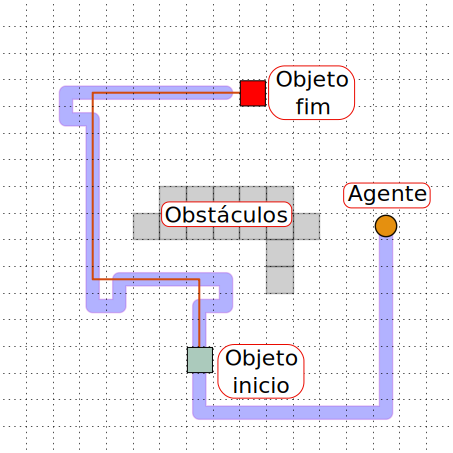
\includegraphics[width=0.42\textwidth]{img/experimentos/mapa_exemplo.png}}
  \caption[Mapa de exemplo do transporte de um objeto por um único agente]{Mapa de exemplo do transporte de um objeto por um único agente, destacando os trajetos realizados tanto pelo objeto quanto pelo agente.}
  \label{fig:result}
\end{figure}

\subsection{Complexidade do Ambiente} % (fold)
\label{sub:complexidade_do_ambiente}

Ao considerar que o transporte dos objetos sofre interferência direta do ambiente em que está sendo realizado, neste estudo, serão utilizados diferentes mapas, com variáveis níveis de complexidade e quantidade de obstáculos, apresentando como o sistema se comporta mediante estas diferentes circunstâncias.

A Figura \ref{fig:cenarios} apresenta exemplos de mapas utilizados nos experimentos desta seção.
Nestes cenários, a quantidade de objetos e robôs foi mantida fixa durante os experimentos (3 robôs e 3 objetos), havendo somente o incremento da complexidade do ambiente, possuindo mais obstáculos, com diferentes configurações.

A principal intenção deste experimento foi demonstrar que o sistema, além de ser capaz de tratar uma diversidade de mapas, não sofre uma grande influência da disposição dos obstáculos no ambiente, apesar de, inevitavelmente, um ambiente com grande restrição de movimentação contribuir em um aumento na distância percorrida pelos agentes.

\begin{figure}[h]
  \centering
  \setlength{\fboxsep}{0pt}
  \begin{subfigure}[t]{0.45\textwidth}
    \centering
    \fbox{\includegraphics[width=\textwidth]{img/experimentos/ambient_1.png}}
    \caption{Ambiente sem obstáculos}
  \end{subfigure}
  \hspace{0.2cm}
  \begin{subfigure}[t]{0.45\textwidth}
    \centering
    \fbox{\includegraphics[width=\textwidth]{img/experimentos/ambient_2.png}}
    \caption{Ambiente com obstáculos dispersos.}
  \end{subfigure}

  \vspace{0.3cm}
  \begin{subfigure}[t]{0.45\textwidth}
    \centering
    \fbox{\includegraphics[width=\textwidth]{img/experimentos/ambient_3.png}}
    \caption{Ambiente com pouca restrição.}
  \end{subfigure}
  \hspace{0.2cm}
  \begin{subfigure}[t]{0.45\textwidth}
    \centering
    \fbox{\includegraphics[width=\textwidth]{img/experimentos/ambient_4.png}}
    \caption{Ambiente com grande restrição.}
  \end{subfigure}

  \caption[Cenários utilizados nos experimentos relacionados à complexidade do ambiente]{Cenários utilizados nos experimentos relacionados à complexidade do ambiente. Os mapas foram criados buscando descrever cenários que possuam diferentes classes de mobilidade, partindo desde o exemplo onde não existem obstáculos, até outros que restringem drasticamente a movimentação tanto de objetos quanto agentes. Cada objeto é demarcado por um identificador numerado, descrevendo o ponto inicial (caixa azul) até seu respectivo destino (caixa vermelha). Os agentes são representados por círculos laranjas.}
  \label{fig:cenarios}
\end{figure}

Os experimentos realizados seguiram as seguintes regras: (i) cada cenário específico foi executado 10 vezes para obtenção dos dados relativos ao tempo médio de planejamento, e (ii) foram realizadas 3 variações aleatórias do posicionamento dos objetos e agentes dentro do ambiente para fins demonstrativos.

Os resultados dos experimentos realizados nestes ambientes podem ser vistos nos gráficos das figuras \ref{fig:cenarios_objeto}, \ref{fig:cenarios_robo}, que demonstram o deslocamento total dos objetos e agentes, respectivamente.
Como pode ser observado, o tamanho do plano de deslocamento dos objetos não segue diretamente um padrão relacionado a complexidade do ambiente, e principalmente à disposição dos mesmos, podendo haver um acréscimo ou descrésimo mediante a relação entre o ponto inicial e final.
O mesmo ocorre com o deslocamento dos robôs, que seguem um modelo similar ao plano dos objetos, quando os planos de transporte são reduzidos, a movimentação dos agentes também é reduzida.

Em contra-partida, o gráfico de tempo de planejamento, demonstrado na Figura \ref{fig:cenarios_tempo}, aponta para o aumento na demanda de tempo necessário durante o planejamento dos planos. Isso era esperado, porque em um ambiente mais restrito, o objeto geralmente deve realizar uma quantidade maior de mudanças de direção durante o transporte, influenciando a etapa de planejamento dos agentes, que devem criar mais planos para cada segmento.
Desta maneira, pode-se concluir que o ambiente certamente gera grande influência sobre o comportamento geral do sistema.

\begin{figure}[h]
  \centering
  \setlength{\fboxsep}{0pt}
  \fbox{\includegraphics[width=0.55\textwidth]{img/experimentos/ambient_objeto.png}}
  \caption{Gráfico do deslocamento do objeto em ambiente com diferentes complexidades. São exemplificados três amostras onde os agentes são dispostos em posições diferentes.}
  \label{fig:cenarios_objeto}
\end{figure}

\begin{figure}[h]
  \centering
  \setlength{\fboxsep}{0pt}
  \fbox{\includegraphics[width=0.55\textwidth]{img/experimentos/ambient_robo.png}}
  \caption{Gráfico de deslocamento dos agentes em cenários com variados graus de restrição de movimentos. Cada amostra demonstrada, representa cenários com agentes em posições distintas.}
  \label{fig:cenarios_robo}
\end{figure}

\begin{figure}[h]
  \centering
  \setlength{\fboxsep}{0pt}
  \fbox{\includegraphics[width=0.55\textwidth]{img/experimentos/ambient_tempo.png}}
  \caption[Gráfico do tempo médio necessário para o planejamento total do sistema]{Gráfico do tempo médio necessário para o planejamento de todos os passos a serem executados durante o transporte em cenários com distintos níveis de complexidade.}
  \label{fig:cenarios_tempo}
\end{figure}

% subsection complexidade_do_ambiente (end)

\clearpage

\subsection{Deslocamento e Tempo de Planejamento dos Agentes} % (fold)
\label{sub:deslocamento_e_templo_de_planejamento_dos_agentes}

Para realizar um estudo específico do planejamento dos agentes, é utilizado um ambiente fixo de complexidade média, como o demonstrado na Figura \ref{fig:ambiente_penalizacao}. Será apresentado um conjunto de experimentos expondo a relação entre a quantidade de robôs e a quantidade de objetos a serem transportados.
Quanto maior a equipe, existe uma maior possibilidade de haver agentes mais aptos para o transporte, porém, como será demonstrado a seguir, em alguns casos, uma equipe maior prejudica a execução total.

% Tal relação se concentra na quantidade de opções (agentes) para transportar um determinado objeto.

\begin{figure}[htpb]
  \centering
  \setlength{\fboxsep}{0pt}
  \fbox{\includegraphics[width=0.5\textwidth]{img/experimentos/ambiente_penalizado.png}}
  \caption[Mapa utilizado nos testes de deslocamento e tempo de planejamento dos agentes]{Mapa utilizado nos testes de deslocamento e tempo de planejamento dos agentes. Neste caso específico, é exibida uma equipe com 6 agentes tendo de transportar 8 objetos dispersos no ambiente.}
  \label{fig:ambiente_penalizacao}
\end{figure}

Esta análise visa demonstrar como o sistema se beneficia do tamanho da equipe além de ilustrar o seu comportamento quando há um certo volume de objetos.
Os experimentos realizados contemplam equipes de 1 até 6 agentes, e o conjunto de objetos variando desde 1 até 8 itens.

Como discutido no Capítulo \ref{cha:metodologia}, o método aqui proposto aplica uma penalização nos planos criados para os objetos e agentes, sempre que existe uma mudança de direção, criando planos mais retilíneos, ou seja, planos que não alternam excessivamente a direção durante o transporte.
Esta penalização se mostrou importante no decorrer da manipulação, pois diminui a distância percorrida pelos agentes, além de minimizar o custo em tempo necessário para o planejamento.

% Exemplo

Para exemplificar visualmente esta diferença, que será discutida a seguir, são apresentados dois gráficos na Figura \ref{fig:ambiente_penalizacao_testes}, que ilustram somente o deslocamento de um agente para transportar 3 objetos, nos casos sem e com a penalização da mudança de direção.
Nos mapas existem 3 áreas destacadas, onde é possível perceber que no exemplo sem a penalidade (Figura \ref{fig:ambiente_penalizacao_sem}), o agente realiza uma série de mudanças de direção que não são realizadas no caso em que há a penalidade (Figura \ref{fig:ambiente_penalizacao_com}).
Desta maneira, o agente tende se deslocar menos durante todo a tarefa de transporte, além de conseguir completar a mesma tarefa em um menor tempo.

\begin{figure}[htpb]
  \centering
  \setlength{\fboxsep}{0pt}

  \begin{subfigure}[t]{0.45\textwidth}
    \centering
    \fbox{\includegraphics[width=\textwidth]{img/experimentos/ambiente_penalizacao_sem.pdf}}
    \caption{Exemplo sem a penalização.}
    \label{fig:ambiente_penalizacao_sem}
  \end{subfigure}
  \hspace{0.2cm}
  \begin{subfigure}[t]{0.45\textwidth}
    \centering
    \fbox{\includegraphics[width=\textwidth]{img/experimentos/ambiente_penalizacao_com.pdf}}
    \caption{Exemplo com a penalização.}
    \label{fig:ambiente_penalizacao_com}
  \end{subfigure}

  \caption[Deslocamento de um agente sem a aplicação da penalização de mudança de direção]{Mapas de deslocamento de um agente demonstrando o transporte de um conjunto de objetos quando é não aplicada a penalização de mudança de direção e o caso onde a penalidade foi utilizada.}
  \label{fig:ambiente_penalizacao_testes}

\end{figure}

Os gráficos a seguir representam o resultado de vários testes realizados, exibindo tanto dados referentes ao deslocamento total dos agentes, quanto ao tempo médio necessário para o planejamento das ações. Foram executados testes tanto aplicando a penalização da mudança de direção quanto sem a mesma. Para uma melhor visualização, foram criados gráficos separando as quantidade de objetos, de 1 a 4 e de 5 a 8, pois a visualização de todos os dados em um só gráfico não permitia uma análise direta devido à escala aplicada nos eixos do gráfico. Cada gráfico exibe em seu eixo horizontal a quantidade de agentes utilizados no experimento, além de representar certas quantidades de objetos sendo transportados por curvas no gráfico.

Os gráficos das figuras \ref{fig:ambiente_penalizacao_deslocamento_sem} e \ref{fig:ambiente_penalizacao_deslocamento_com} demonstram o somatório do deslocamento de todos os agentes, respectivamente os casos onde não foi aplicada a penalização e quando a mesma foi utilizada.
O mesmo pode ser visto nas figuras \ref{fig:ambiente_penalizacao_tempo_sem} e \ref{fig:ambiente_penalizacao_tempo_com}, porém exibindo os dados de tempo de planejamento, no cenário sem e com a penalização.
% Especificamente o gráfico da Figura \ref{fig:ambiente_penalizacao_deslocamento_sem} exibe o caso onde não há penalização, e a Figura \ref{fig:ambiente_penalizacao_deslocamento_penalizado}, o caso com penalização.

% DESLOCAMENTO

\begin{figure}[h]
  \centering
  \setlength{\fboxsep}{0pt}
  \begin{subfigure}[t]{0.49\textwidth}
    \centering
    \fbox{\includegraphics[width=\textwidth]{img/experimentos/penalizacao/penalizado_des_sem_1_4.png}}
    \caption{1 a 4 objetos.}
    % \label{fig:ambiente_penalizacao_deslocamento_normal}
  \end{subfigure}
  \begin{subfigure}[t]{0.49\textwidth}
    \centering
    \fbox{\includegraphics[width=\textwidth]{img/experimentos/penalizacao/penalizado_des_sem_5_8.png}}
    \caption{5 a 8 objetos.}
    % \label{fig:ambiente_penalizacao_deslocamento_penalizado}
  \end{subfigure}
  % Gráficos com o do deslocamento total dos agentes em diferentes configurações de ambientes de teste. Cada curva representa uma certa quantidade de objetos a serem transportados pela equipe, partindo de 1 objeto até 8.
  % Gráficos com o deslocamento total dos agentes, nos casos em que a penalização de mudança de direção não foi aplicada. Cada curva representa uma quantidade distinta de objetos, de 1 a 8.
  \caption[Deslocamento de um agente utilizando a penalização de mudança de direção]{Deslocamento total dos agentes quando não foi aplicada a penalidade de mudança de direção.}
  \label{fig:ambiente_penalizacao_deslocamento_sem}
\end{figure}

\begin{figure}[h]
  \centering
  \setlength{\fboxsep}{0pt}

  \begin{subfigure}[t]{0.49\textwidth}
    \centering
    \fbox{\includegraphics[width=\textwidth]{img/experimentos/penalizacao/penalizado_des_com_1_4.png}}
    \caption{1 a 4 objetos.}
    % \label{fig:ambiente_penalizacao_deslocamento_normal}
  \end{subfigure}
  \begin{subfigure}[t]{0.49\textwidth}
    \centering
    \fbox{\includegraphics[width=\textwidth]{img/experimentos/penalizacao/penalizado_des_com_5_8.png}}
    \caption{5 a 8 objetos.}
    % \label{fig:ambiente_penalizacao_deslocamento_penalizado}
  \end{subfigure}
  % Gráficos com o do deslocamento total dos agentes em diferentes configurações de ambientes de teste. Cada curva representa uma certa quantidade de objetos a serem transportados pela equipe, partindo de 1 objeto até 8.
  % Gráficos representando o deslocamento total dos agentes durante o transporte com a aplicação da penalização da mudança de direção. Cada curva uma quantidade de objetos transportados, de 1 a 8.
  \caption{Deslocamento total dos agentes com a aplicação da penalidade de mudança de direção.}
  \label{fig:ambiente_penalizacao_deslocamento_com}
\end{figure}

% DESLOCAMENTO

% TEMPO

\begin{figure}[h]
  \centering
  \setlength{\fboxsep}{0pt}

  \begin{subfigure}[t]{0.49\textwidth}
    \centering
    \fbox{\includegraphics[width=\textwidth]{img/experimentos/penalizacao/penalizado_tem_sem_1_4.png}}
    \caption{1 a 4 objetos.}
    % \label{fig:ambiente_penalizacao_tempo_normal}
  \end{subfigure}
  \begin{subfigure}[t]{0.49\textwidth}
    \centering
    \fbox{\includegraphics[width=\textwidth]{img/experimentos/penalizacao/penalizado_tem_sem_5_8.png}}
    \caption{5 a 8 objetos.}
    % \label{fig:ambiente_penalizacao_tempo_penalizado}
  \end{subfigure}
  % Gráficos representativos do tempo de planejamento dos agentes em cenários com diferentes quantidades de objetos e robôs. Cada curva representa uma certa quantidade de objetos.
  \caption{Tempo de planejamento dos agentes sem a aplicação da penalidade de mudança na direção.}
  \label{fig:ambiente_penalizacao_tempo_sem}
\end{figure}

\begin{figure}[h]
  \centering
  \setlength{\fboxsep}{0pt}

  \begin{subfigure}[t]{0.49\textwidth}
    \centering
    \fbox{\includegraphics[width=\textwidth]{img/experimentos/penalizacao/penalizado_tem_com_1_4.png}}
    \caption{1 a 4 objetos.}
    % \label{fig:ambiente_penalizacao_tempo_normal}
  \end{subfigure}
  \begin{subfigure}[t]{0.49\textwidth}
    \centering
    \fbox{\includegraphics[width=\textwidth]{img/experimentos/penalizacao/penalizado_tem_com_5_8.png}}
    \caption{5 a 8 objetos.}
    % \label{fig:ambiente_penalizacao_tempo_penalizado}
  \end{subfigure}
  % Gráficos representativos do tempo de planejamento dos agentes em cenários com diferentes quantidades de objetos e robôs. Cada curva representa uma certa quantidade de objetos.
  \caption{Tempo de planejamento dos agentes com a aplicação da penalidade de mudança na direção.}
  \label{fig:ambiente_penalizacao_tempo_com}
\end{figure}

% TEMPO

Ao analisar os gráficos de deslocamento, é possível notar que nos casos em que não há a penalização da mudança de direção, o sistema não se beneficia tanto da quantidade de agente, que contrariamente ao esperado, aumenta a distância percorrida quando a equipe aumenta de tamanho.
Comportamento este que não é observado quando é a aplicada a penalização, em que a tendência do sistema é necessitar de uma menor quantidade total de deslocamento para realizar o transporte dos objetos.
A diminuição nos trajetos era esperada, considerando que uma maior quantidade de agentes garante uma maior diversidade de opções para transportar um determinado objeto, criando mais chances de existirem robôs com planos melhores, contribuindo para minimizar a movimentação geral.

Apesar da diminuição na movimentação dos agentes com a penalização, em alguns casos, é notado que o aumento da quantidade de agentes, mesmo que sutil, faz com que os agentes andem mais que nos casos com uma menor equipe, como na situação do transporte de 8 objetos por 4 e 5 agentes.
Isso é explicado pelo fato do algoritmo de alocação de tarefas (Seção \ref{sec:aloca_o_de_tarefas}) sempre alocar tarefas para todos os agentes, mesmo que a melhor configuração fosse deixar um determinado robô sem nenhuma tarefa, afetando assim o deslocamento total dos agentes.
Mesmo com este acréscimo, deve ser lembrado que com mais agentes, executando mais tarefas ao mesmo tempo, o tempo de execução total da tarefa reduzirá.

Em relação ao tempo de planejamento, um efeito contrário é observado. Seja com o aumento no número de objetos ou no número de agentes, o sistema tende a consumir mais tempo para planejar todas as rotas necessárias para o transporte.
O aumento no número de objetos faz com que os agentes tenham mais opções de planos a executar, já o aumento no número de agentes aumenta a quantidade de possíveis robôs para executar o transporte de um objeto, além de uma necessidade maior de tempo para que toda a equipe entre em acordo sobre quais tarefas executar.
Mesmo com este comportamento, observa-se nos gráficos onde há a aplicação da penalidade, o tempo necessário para o planejamento é sempre menor ou bastante aproximado dos casos em que não é aplicada, demonstrando como esta estratégia contribui para o melhoramento da performance do sistema.

% Ao analisar os gráficos de deslocamento, dois pontos podem ser notados: (i) conforme o número de agentes na equipe aumenta, a distância total percorrida decai, isto porque existe uma maior chance de haver um agente próximo ao um determinado objeto, retirando a responsabilidade de outro robô distante do mesmo e assim minimizando todos os planos; e (ii) na presença de penalização é perceptível que os planos em sua maioria são minimizados, isto é explicado quando o agente não necessita empurrar o objeto de diferentes posições, criando menos planos de preparação e consequentemente, reduzindo o espaço de deslocamento.

% Apesar disso, um efeito contrário é observado na dimensão de tempo do planejamento. Quando existe uma equipe maior de agentes e maior número de objetos, maior é o tempo necessário para que todos planejem e entrem em acordo sobre as tarefas a serem realizadas.

Estes fatores são interessantes de serem estudados pois ocasionam um \emph{trade-off} entre a quantidade de robôs a ser utilizada, o tempo de planejamento e o ganho em deslocamento total.
Encontrar a melhor combinação destes valores não foi objetivo deste trabalho, mas sim demonstrar que cada uma destas variáveis influencia diretamente na performance total do sistema.

% subsection deslocamento_e_templo_de_planejamento_dos_agentes (end)

\subsection{Função de Utilidade} % (fold)
\label{sub:fun_o_de_utilidade}

Durante o desenvolvimento do método, chegou-se à conclusão que seria possível criar um sistema no qual fosse possível configurar os algoritmos de planejamento de modo a atender diferentes demandas, criando planos que fossem ou mais rápidos de serem executados, ou mesmo com um menor custo energético para realização.

Esta configuração é possível através de um artifício na heurística utilizada no algoritmo modificado A* utilizado nas etapas de criação dos planos de movimentação.
A função heurística descrita na Seção \ref{sub:fun_o_de_avalia_o} exerce sua influência para modificar o plano.

Neste sentido, foram realizados experimentos em um mapa simples, como o demonstrado a seguir na Figura \ref{fig:utility_function_graph}, modificando as constantes de ponderação em cada dimensão analisada, tempo e energia. A Tabela \ref{table:utility_function_graph} expõe os pesos utilizado em cada experimento.

\begin{table}
    \centering
    \caption[Tabela com as variações nos pesos da função de utilidade]{Tabela com as variações nos pesos utilizados para realização de testes aplicados na função de utilidade durante a fase de planejamento dos objetos.}
    \label{table:utility_function_graph}
    \begin{tabular}{|c|c|c|}
    \hline
    Experimento & Tempo & Energia \\ \hline
    1        & 1     & 0       \\ \hline
    2        & 0     & 1       \\ \hline
    3        & 0.5   & 0.5     \\ \hline
    \end{tabular}
\end{table}

Um fato importante de ser mencionado é que estes experimentos, apesar de serem reflexo da influência da função de utilidade, só possuem sentido levando em consideração as características dos agentes utilizados durante o planejamento.
Estes parâmetros são utilizados durantes os cálculos para decidir a utilidade de certa ação de movimento realizada por cada tipo de agente, e assim, decidir o melhor caminho que atenda às configurações previamente estabelecidas pelas constantes de ponderação.

Os experimentos ilustrados nos mapas da Figura \ref{fig:utility_function_graph}, utilizam dois tipos de agentes, um terrestre e outro aéreo. Para averiguar as características dos mesmo, foram realizados dois tipos de testes: (i) a velocidade média de deslocamento entre dois pontos fixos do ambiente, considerando somente a movimentação em linha reta, e (ii) o tempo médio de duração da bateria em uso contínuo.
Uma vez realizados estas provas, a tabela \ref{table:caracteristicas} apresenta os valores estimados para cada tipo de agente.
Estes dados são demonstrados de forma unitária, ou seja, o agente com melhor performance em uma determinada característica possui valor 1, e o outro agente possui um valor determinado em quantas vezes o mesmo é pior naquela propriedade.
Estes dados não são fixos ou finais, pois estão diretamente relacionados ao tipos de agentes utilizados durantes os testes, podendo haver uma grande diferença se outras plataformas robótica fossem utilizadas durante as provas.

\begin{table}
    \centering
    \caption[Dados referente às características dos tipos de agentes]{Dados referente às características dos tipos de agentes utilizados durante os experimentos da função de utilidade.}
    \label{table:caracteristicas}
    \begin{tabular}{|c|c|c|}
    \hline
    Tipo      & Energia & Tempo \\ \hline
    Terrestre & 1       & 8     \\ \hline
    Aéreo     & 12      & 1     \\ \hline
    \end{tabular}
\end{table}

\begin{figure}[htpb]
  \centering
  \setlength{\fboxsep}{0pt}

  \begin{subfigure}[t]{0.315\textwidth}
    \centering
    \fbox{\includegraphics[width=\textwidth]{img/experimentos/utility_func_time.png}}
    \caption{Experimento 1}
    % Plano do objeto favorecendo o tempo de execução. Variação 1.
    \label{fig:utility_function_time}
  \end{subfigure}
  \hspace{0.1cm}
  \begin{subfigure}[t]{0.315\textwidth}
    \centering
    \fbox{\includegraphics[width=\textwidth]{img/experimentos/utility_func_energy.png}}
    \caption{Experimento 2}
    % Plano do objeto priorizando o baixo custo energético. Variação 2.
    \label{fig:utility_function_energy}
  \end{subfigure}
  \hspace{0.1cm}
  \begin{subfigure}[t]{0.315\textwidth}
    \centering
    \fbox{\includegraphics[width=\textwidth]{img/experimentos/utility_func_mid.png}}
    \caption{Experimento 3}
    % Plano do objeto realizando uma mediação entre tempo e energia. Variação 3.
    \label{fig:utility_function_mid}
  \end{subfigure}

  \caption[Exemplos de planos de movimentação de um objeto com diferentes pesos na função de utilidade]{Exemplos de planos de movimentação de um objeto mediante a troca das constantes de ponderação na função de utilidade utilizada como heurística do planejador. O caminho demarcado em laranja representa um trajeto aéreo, enquanto o lilás é terrestre.}
  \label{fig:utility_function_graph}

\end{figure}

Mediante os dados expostos, é possível observar como a mudança nos pesos da função de utilidade é capaz de atuar sobre os planos criados, tornando o método apresentado flexível, passível de ser configurado para atender a diferentes necessidades.

% subsection fun_o_de_utilidade (end)

\subsection{Sequenciamento do Transporte} % (fold)
\label{sub:tipo_de_transporte}

Um importante fator durante a ação de transporte de objetos é a escolha da sequência na qual estes objetos serão manipulados, pois, uma ordenação mal determinada pode levar os agentes a transcorrer grandes distâncias para realizar o deslocamento.

Neste experimento serão realizados experimentos comparando dois tipos de transporte: (i) sequencial -- na qual os objetos são manipulados em uma ordem pré-definida, não avaliando qualquer custo excessivo associado ao deslocamento dos agentes, e (ii) oportunista -- onde é avaliado o melhor objeto a ser transportado em um determinado momento baseado na localização do agente, procurando sempre minimizar a distância percorrida.

De forma demonstrativa, são exibidos na Figura \ref{fig:figure_simple_smart} dois gráficos com o deslocamento de um agente realizando o transporte de 3 objetos, onde são destacadas as áreas de maior discrepância entre os resultados do tipo de transporte.
O mapa utilizado durante este experimento é similar ao da Figura \ref{fig:cenario_sequencial_oportunista}.
Como pode ser observado, durante o transporte sequencial o agente realiza planos mais longos, pois esta métrica (tamanho do plano) não é levada em consideração durante a escolha do objeto, em comparação ao transporte oportunista, que sempre visa o objeto com melhor custo, este apresenta um comportamento com menor distâncial total percorrida nos planos.

O mapa apresentado na Figura \ref{fig:cenario_sequencial_oportunista} ilustra o ambiente no qual os demais experimentos foram realizados, nos quais também um agente foi utilizado, o que proporciona uma melhor visualização do seu deslocamento referente à sequência do transporte.

\begin{figure}[h]
  \centering
  \setlength{\fboxsep}{0pt}

  \begin{subfigure}[t]{0.45\textwidth}
    \centering
    \fbox{\includegraphics[width=\textwidth]{img/experimentos/figure_simple.pdf}}
    \caption{Transporte sequencial}
    \label{fig:figure_simple}
  \end{subfigure}
  \hspace{0.2cm}
  \begin{subfigure}[t]{0.45\textwidth}
    \centering
    \fbox{\includegraphics[width=\textwidth]{img/experimentos/figure_smart.pdf}}
    \caption{Transporte oportunista}
    \label{fig:figure_smart}
  \end{subfigure}

  \caption[Resultado do transporte de 3 objetos por um agente]{Resultado do transporte de 5 objetos por um agente utilizando o método sequencial e o oportunista.}
  \label{fig:figure_simple_smart}

\end{figure}

\begin{figure}[h]
  \centering
  \setlength{\fboxsep}{0pt}
  \fbox{\includegraphics[width=0.5\textwidth]{img/experimentos/mapa_sequencial_oportunista.png}}
  \caption[Mapa utilizado nos testes sequencial e oportunista]{Mapa utilizado para avaliar a diferenciação entre os tipos de atitudes no transporte, sequencial e oportunista.}
  \label{fig:cenario_sequencial_oportunista}
\end{figure}

\begin{figure}[h]
  \centering
  \setlength{\fboxsep}{0pt}
  \fbox{\includegraphics[width=0.8\textwidth]{img/experimentos/sequencial_oportunista_deslocamento.png}}
  \caption[Deslocamento do robô mediante nos transportes sequencial e oportunista]{Deslocamento do robô mediante a adição de objetos utilizando dois tipos de transporte, sequencial e oportunista.}
  \label{fig:cenario_sequencial_oportunista_deslocamento}
\end{figure}

\begin{figure}[h]
  \centering
  \setlength{\fboxsep}{0pt}
  \fbox{\includegraphics[width=0.8\textwidth]{img/experimentos/sequencial_oportunista_tempo.png}}
  \caption[Tempo de planejamento do agente nos transporte sequencial e oportunista]{Tempo de planejamento do agente nas duas técnicas de transporte, sequencial e oportunista.}
  \label{fig:cenario_sequencial_oportunista_tempo}
\end{figure}

A Figura \ref{fig:cenario_sequencial_oportunista_deslocamento} demonstra um gráfico comparativo entre as distâncias percorridas pelo agente quando o número de objetos a ser transportado aumenta. Mesmo que os planos se tornem mais longos com a adição de objetos, que é um fato esperado, é possível perceber que o método oportunista faz um melhor uso da posição do robô, proporcionando uma menor travessia total e assim economizando tanto tempo como energia, pois estes custos estão diretamente relacionados ao tamanho do plano executado.

Apesar da vantagem apresentada, como é demonstrado no gráfico da Figura \ref{fig:cenario_sequencial_oportunista_tempo}, o tempo necessário de planejamento no caso oportunista apresenta um comportamento de crescimento muito superior à técnica sequencial.
Este desempenho é justificado ao considerar que o agente deve decidir qual o melhor objeto a transportar, e para tal, deve considerar planos de transporte para todos os objetos ainda não transportados, gerando uma maior demanda de tempo nesta etapa, diferente da técnica sequencial, na qual somente o objeto atualmente sendo manipulado é tido como base pra realização do planejamento.

Porém, é interessante ressaltar que, apesar do grande gasto de tempo durante o planejamento, este não afeta drasticamente o gasto energético do agente, pois o mesmo não está em movimentação, o que justifica o uso da técnica oportunista, considerando que o ganho proporcionado por um menor plano é superior ao ganho quando o planejamento é executado rapidamente.

\section{Ambiente Simulado} % (fold)
\label{sub:ambiente_simulado}

Para realização dos testes simulados, foi utilizado o \emph{Robot Operating System (ROS)}\footnote{www.ros.org}, que é um conjunto bibliotecas para desenvolvimento de plataformas autônomas largamente utilizado tanto em pesquisas quanto em aplicações comerciais. Especificamente a versão \emph{Indigo} foi utilizada na implementação.
Este sistema abstrai as camadas de envio e recebimento de dados, provendo acesso aos sensores e atuadores de diversas plataformas robóticas.

Os algoritmos desenvolvidos foram testados no ambiente de simulação \emph{Gazebo}\footnote{http://gazebosim.org/}. O mesmo já possui integração direta com o \emph{ROS}, capaz de simular a dinâmica entre corpos virtuais utilizando diferentes motores de física (\emph{ODE}, \emph{Bullet}, \emph{Simbody}, \emph{DART}), além de implementar uma diversidade de sensores (câmeras RGB-D, laser, torque) e possuir vários modelos pré-existentes para criação de ambientes realísticos, tanto de robôs, mas também inclui ferramentas, casas, véículos, dentre outros.

Para uma demonstração da técnica apresentada por este trabalho, serão documentados dois experimentos simulados, visando exemplificar o processo de coordenação entre diferentes agentes. Serão apresentados dois casos do transporte de um objeto: (i) dois agentes terrestres e (ii) um agente terrestre e outro aéreo.

A Figura \ref{fig:maps} demonstra os ambientes de trabalho construídos para a simulação. Neles é possível observar a disposição do objeto a ser transportado, bem como dos agentes e obstáculos.

\begin{figure}[h]
  \centering
  \setlength{\fboxsep}{0pt}

  \begin{subfigure}[t]{0.45\textwidth}
    \centering
    \includegraphics[width=\textwidth]{img/experimentos/sim_map1.png}
    \caption{Dois agentes terrestres.}
  \end{subfigure}
  \hspace{0.2cm}
  \begin{subfigure}[t]{0.45\textwidth}
    \centering
    \includegraphics[width=\textwidth]{img/experimentos/sim_map2.png}
    \caption{Um agente terrestre e outro aéreo.}
  \end{subfigure}

  \caption{Ambientes de trabalho utilizados durante os experimentos simulados.}
  \label{fig:maps}

\end{figure}

A Figura \ref{fig:sim_ground} ilustra o transporte de um objeto por uma equipe de dois agentes terrestres. Os agentes representados são da plataforma \emph{iRobot Create}, robô diferencial com dimensões de 33cm de diâmetro e 12cm de altura, capazes de executar somente a ação de \emph{PUSH} no objeto.
Cada sub-figura ilustra um determinado estado do sistema com seu respectivo tempo de ocorrência.

\begin{figure}[ht!]
  \centering
  \setlength{\fboxsep}{0pt}

  \begin{subfigure}[t]{0.45\textwidth}
    \centering
    \fbox{\includegraphics[width=\textwidth]{img/experimentos/sim_001.png}}
    \caption{t=1s}
    \label{fig:sim_1}
  \end{subfigure}
  \hspace{0.2cm}
  \begin{subfigure}[t]{0.45\textwidth}
    \centering
    \fbox{\includegraphics[width=\textwidth]{img/experimentos/sim_044.png}}
    \caption{t=44s}
    \label{fig:sim_44}
  \end{subfigure}

  \begin{subfigure}[t]{0.45\textwidth}
    \centering
    \fbox{\includegraphics[width=\textwidth]{img/experimentos/sim_078.png}}
    \caption{t=78s}
    \label{fig:sim_78}
  \end{subfigure}
  \hspace{0.2cm}
  \begin{subfigure}[t]{0.45\textwidth}
    \centering
    \fbox{\includegraphics[width=\textwidth]{img/experimentos/sim_139.png}}
    \caption{t=139s}
    \label{fig:sim_139}
  \end{subfigure}

  \begin{subfigure}[t]{0.45\textwidth}
    \centering
    \fbox{\includegraphics[width=\textwidth]{img/experimentos/sim_180.png}}
    \caption{t=180s}
    \label{fig:sim_180}
  \end{subfigure}
  \hspace{0.2cm}
  \begin{subfigure}[t]{0.45\textwidth}
    \centering
    \fbox{\includegraphics[width=\textwidth]{img/experimentos/sim_200.png}}
    \caption{t=200s}
    \label{fig:sim_200}
  \end{subfigure}

  \begin{subfigure}[t]{0.45\textwidth}
    \centering
    \fbox{\includegraphics[width=\textwidth]{img/experimentos/sim_230.png}}
    \caption{t=230s}
    \label{fig:sim_230}
  \end{subfigure}
  \hspace{0.2cm}
  \begin{subfigure}[t]{0.45\textwidth}
    \centering
    \fbox{\includegraphics[width=\textwidth]{img/experimentos/sim_250.png}}
    \caption{t=250s}
    \label{fig:sim_250}
  \end{subfigure}

  \caption{Exemplo de transporte por dois agentes em um ambiente simulado.}
  \label{fig:sim_ground}

\end{figure}

Neste exemplo de execução, o agente mais próximo do objeto será alocado para realizar o primeiro segmento do transporte do objeto através do corredor formado pelos obstáculos (figuras \ref{fig:sim_1} a \ref{fig:sim_139}).
Considerando que para continuar a execução do transporte, o primeiro agente deve andar uma grande distância, o segundo agente assume o objeto para realização do segundo segmento, levando-o até a posição final, demarcada por uma caixa verde semitransparente (figuras \ref{fig:sim_180} a \ref{fig:sim_250}).

No outro ambiente simulado apresentado na Figura \ref{fig:sim_aerial}, é demonstrado o transporte do objeto em questão utilizando agentes de tipos diferentes, um terrestre, da mesma plataforma utilizada anteriormente (\emph{iRobot Create}), e um aéreo, que é representado por um robô genérico no modelo \emph{quadrotor}, este tipo de agente foi escolhido por sua capacidade de pairar, sendo capaz de pegar o objeto ainda no ar utilizando a ação de \emph{GRASP}.

Diferente do ambiente anterior, neste novo cenário o objeto não tem acesso direto ao seu destino por vías terrestres, sendo necessário o uso do agente aéreo.
Em um primeiro momento, visto nas figuras \ref{fig:sim_aerial_1} até \ref{fig:sim_aerial_668}, o agente terrestre transporta o objeto até o local mais próximo possível de sua posição final evitando o objeto colida com os obstáculos, em seguida (figuras \ref{fig:sim_aerial_687} a \ref{fig:sim_aerial_742}) o agente aéreo é acionado, indo até a posição atual do objeto, realiza a ação de \emph{GRASP} e o leva até a pose final designada.

\begin{figure}[ht!]
  \centering
  \setlength{\fboxsep}{0pt}

  \begin{subfigure}[t]{0.45\textwidth}
    \centering
    \fbox{\includegraphics[width=\textwidth]{img/experimentos/sim_aerial/sim_001.png}}
    \caption{t=1s}
    \label{fig:sim_aerial_1}
  \end{subfigure}
  \hspace{0.2cm}
  \begin{subfigure}[t]{0.45\textwidth}
    \centering
    \fbox{\includegraphics[width=\textwidth]{img/experimentos/sim_aerial/sim_139.png}}
    \caption{t=139s}
    \label{fig:sim_aerial_139}
  \end{subfigure}

  \begin{subfigure}[t]{0.45\textwidth}
    \centering
    \fbox{\includegraphics[width=\textwidth]{img/experimentos/sim_aerial/sim_459.png}}
    \caption{t=459s}
    \label{fig:sim_aerial_459}
  \end{subfigure}
  \hspace{0.2cm}
  \begin{subfigure}[t]{0.45\textwidth}
    \centering
    \fbox{\includegraphics[width=\textwidth]{img/experimentos/sim_aerial/sim_566.png}}
    \caption{t=566s}
    \label{fig:sim_aerial_566}
  \end{subfigure}

  \begin{subfigure}[t]{0.45\textwidth}
    \centering
    \fbox{\includegraphics[width=\textwidth]{img/experimentos/sim_aerial/sim_668.png}}
    \caption{t=668s}
    \label{fig:sim_aerial_668}
  \end{subfigure}
  \hspace{0.2cm}
  \begin{subfigure}[t]{0.45\textwidth}
    \centering
    \fbox{\includegraphics[width=\textwidth]{img/experimentos/sim_aerial/sim_687.png}}
    \caption{t=687s}
    \label{fig:sim_aerial_687}
  \end{subfigure}

  \begin{subfigure}[t]{0.45\textwidth}
    \centering
    \fbox{\includegraphics[width=\textwidth]{img/experimentos/sim_aerial/sim_700.png}}
    \caption{t=700s}
    \label{fig:sim_aerial_700}
  \end{subfigure}
  \hspace{0.2cm}
  \begin{subfigure}[t]{0.45\textwidth}
    \centering
    \fbox{\includegraphics[width=\textwidth]{img/experimentos/sim_aerial/sim_713.png}}
    \caption{t=713s}
    \label{fig:sim_aerial_713}
  \end{subfigure}

  \begin{subfigure}[t]{0.45\textwidth}
    \centering
    \fbox{\includegraphics[width=\textwidth]{img/experimentos/sim_aerial/sim_720.png}}
    \caption{t=720s}
    \label{fig:sim_aerial_720}
  \end{subfigure}
  \hspace{0.2cm}
  \begin{subfigure}[t]{0.45\textwidth}
    \centering
    \fbox{\includegraphics[width=\textwidth]{img/experimentos/sim_aerial/sim_742.png}}
    \caption{t=742s}
    \label{fig:sim_aerial_742}
  \end{subfigure}

  \caption{Exemplo de transporte utilizando um agente terrestre e um aéreo.}
  \label{fig:sim_aerial}

\end{figure}

Mediante estes exemplos, é possível ver todas as etapas anteriormente discutidas, havendo o planejamento para o objeto, os agentes realizam seus próprios planejamento e se coordenam de modo a transportar o objeto da melhor maneira possível, respeitando as restrições impostas pelo ambiente.

% Algoritmo de Controle

O controle dos agentes durante a movimentação no ambiente de trabalho foi realizado utilizando um conjunto de algoritmos separados em dois níveis: (i) controlador de navegação, que mantém um registro de todas as posições no ambiente de trabalho que o agente deve percorrer para completar o plano previamente criado, além de gerenciar o envio de novos pontos de destino sempre que detectar a chegada do agente a uma posição previamente enviada; (ii) controlador de velocidades, este recebe um ponto de destino do controlador de navegação, e baseado na posição atual do agente, aplica um controlador PI (proporcional-integrativo) para realizar a movimentação do agente para a posição requerida.

Para ambos os agentes, o algoritmo do controlador de navegação utilizado é o mesmo, pois é necessário somente o repasse dos pontos de destino, porém o controlador de baixo nível (velocidades) é diferenciado, considerando que os agentes possuem maneiras de movimentação distintas.
Os Algoritmos \ref{alg:aerial_vel} e \ref{alg:land_vel} demonstram sucintamente estes controladores, respectivamente do agente aéreo e terrestre.

\begin{algorithm}[h]
  \caption{AerialVelocityController(goal\_pose, last\_cmd, vertical\_lim, P, I)}
  \label{alg:aerial_vel}
  \begin{algorithmic}[1]
    \STATE{current\_pose $\leftarrow$ get\_current\_pose()}
    \STATE{current\_orientation $\leftarrow$ get\_orientation(current\_pose)}
    \STATE{}
    \STATE{diff\_x $\leftarrow$ goal\_pose[x] - current\_pose[x]}
    \STATE{diff\_y $\leftarrow$ goal\_pose[y] - current\_pose[y]}
    \STATE{diff\_z $\leftarrow$ goal\_pose[z] - current\_pose[z]}
    \STATE{}
    \STATE{angular\_vel $\leftarrow$ P * current\_orientation + I * last\_cmd[angle]}
    \STATE{}
    \IF{abs(diff\_z) $>$ vertical\_lim}
      \STATE{linear\_vel\_x $\leftarrow 0$}
      \STATE{linear\_vel\_y $\leftarrow 0$}
    \ELSE
      \STATE{linear\_vel\_x $\leftarrow$ P * diff\_x + I * last\_cmd[x]}
      \STATE{linear\_vel\_y $\leftarrow$ P * diff\_y + I * last\_cmd[y]}
    \ENDIF
    \STATE{linear\_vel\_z $\leftarrow$ P * diff\_z + I * last\_output[z]}
    \RETURN{[linear\_vel\_x, linear\_vel\_y, linear\_vel\_z, angular\_vel]}
  \end{algorithmic}
\end{algorithm}

\begin{algorithm}[h]
  \caption{AerialVelocityController(goal\_pose, last\_cmd, angular\_lim, P, I)}
  \label{alg:land_vel}
  \begin{algorithmic}[1]
    \STATE{current\_pose $\leftarrow$ get\_current\_pose()}
    \STATE{current\_orientation $\leftarrow$ get\_orientation(current\_pose)}
    \STATE{}
    \STATE{diff\_orientation $\leftarrow$ angle\_between\_poses(current\_pose, goal\_pose)}
    \STATE{diff\_distance $\leftarrow$ distance\_between\_poses(current\_pose, goal\_pose)}
    \STATE{}
    \IF{abs(diff\_orientation) $>=$ angular\_lim}
      \STATE{linear\_vel $\leftarrow 0$}
    \ELSE
      \STATE{linear\_vel $\leftarrow$ P * diff\_distance + I * last\_cmd[linear]}
    \ENDIF
    \STATE{angular\_vel $\leftarrow$ P * diff\_orientation + I * last\_cmd[angular]}
    \RETURN{[linear\_vel, angular\_vel]}
  \end{algorithmic}
\end{algorithm}

O Algoritmo \ref{alg:aerial_vel}, demonstra o controle para o agente aéreo.
Em um primeiro momento, o mesmo guarda referências para sua posição e orientação atual (referente ao sistema de coordenada do mundo), e calcula a diferença entre sua atual localidade até o ponto de destino.
Considerando que não há necessidade de rotação do agente, o mesmo deve manter uma orientação fixa próximo ao valor $0$, assim é calculada a velocidade angular necessária para correção de possíveis variações (linha $8$).
Nas demais linhas, são calculas as velocidades lineares de movimentação em três dimensões (x, y, z), observando para um detalhe na linha 10, que faz uso da constante $vertical\_lim$ para delimitar uma distância mínima entre a altitude do agente e a altitude de destino, fazendo com o mesmo se movimente no plano (x, y) somente quando este limiar for atingido.
Sem este detalhe de implementação, o agente movimentáva-se nos três eixos simultaneamente, ocasionando em colisões descenessárias com o ambiente.

Para o agente terrestre, foi utilizado o Algoritmo \ref{alg:land_vel}, que funciona de forma similar ao demonstrado anteriormente, porém de forma mais simples. Baseado na posição e orientação atual, o agente calcula a diferença de ângulo até o ponto de destino, aplicando a função $\arctan$, além da distância entre os mesmos.
Análogo ao limiar de altitude, o agente terrestre utiliza a constante $angular\_lim$ para delimitar uma diferença de angulo mínimo para que o robô possa se mover. Durante os testes, fora utilizado um valor reduzido para tal constante, ocasionando em uma ausência de curvas por parte do agente, de modo que o mesmo primeiramente realiza um alinhamento em direção à posição de destino e só então realiza a movimentação.

Em ambos os algoritmos, os valores passados através variável $last\_cmd$, são todos aqueles calculados durante a ultima iteração do mesmo, controlado externamento pelo algoritmo de navegação.

\subsection{Ambiente Real} % (fold)
\label{sub:ambiente_real}

Os experimentos reais foram realizados utilizando somente agentes terrestres, em um espaço de área aproximada de 2m x 2m situado no laboratório de Visão Computacional e Robótica (VeRLab)\footnote{\url{http://www.verlab.dcc.ufmg.br/}}.
O mesmo controlador anteriormente descrito foi utilizado, com pequenos ajustes nos valores das constantes para atender às variações do ambiente real.

A metodologia apresentada considera que a localização de todos os agentes, objetos e obstáculos no ambiente é conhecida durante a missão de transporte, para tanto, a localização de tais itens foi realizada utilizando marcadores fiduciais que identificam unicamente cada um e são reconhecidos por uma câmera posicionada acima da área de trabalho, sendo capaz de detectar a posição de cada marcador e informar ao sistema estas informações em tempo real.

A plataforma robótica utilizada nos experimentos é do modelo \emph{ePuck}\footnote{\url{http://www.e-puck.org/}}, robô diferencial, com 70mm de diâmetro e 150g, controlado através de comunicação \emph{bluetooth}.
Esta robô é capaz de se movimentar, além de possuir alguns sensores, como uma câmera, um conjunto de infra-vermelhos para detecção de obstáculos, além de \emph{encoders} para as rodas.
A Figura \ref{fig:epucks} exemplifica o agente utilizado durante o experimentos.

O ambiente de trabalho montado para realização deste experimento consistia na utilização de três robôs \emph{ePuck}s, um objeto a ser transportado, e um conjunto arbitrário de obstáculos dispostos no ambiente, como é demonstrado na Figura \ref{fig:real_workspace}.
Como apresentado na figura, os agentes foram colocados em uma região à parte do ambiente, passíveis de serem utilizados durante o transporte.
O objeto a ser transportado é considerado possuindo peso e resistência desprezíveis, por ser constituído de uma espuma de baixa densidade e apresentar baixa taxa atrito com a superfície na qual o teste está sendo realizado, além de possuir a mesma dimensão (largura e comprimento) que os agentes.
Os agentes tem por objetivo levar o objeto de sua posição inicial, assinala em verde, para a posição final, destacada em vermelho.

A Figura \ref{fig:real} demonstra a execução da missão de transporte pelos três agentes, considerando que as etapas de planejamento de caminhos do objetos (destacada pelo caminho na cor branca na Figura \ref{fig:real_workspace}, possuindo 3 segmentos) e dos agentes, além da alocação de tarefas já foram realizadas enquanto os agentes permaneciam em suas respectivas posições iniciais.
Como pode ser observado, o agente 1 é selecionado para iniciar o transporte, enquanto os demais agentes se movimentam para esperar sua vez.
Assim que o agente transporta objeto através do primeiro segmento (S1) na Figura \ref{fig:real_5} o agente 2 torna-se o responsável pelo transporte através do segmento S2, até que a missão é repassada para o agente 3 como demonstrado na Figura \ref{fig:real_7}, que termina a movimentação do objeto até a posição final passando pelo segmento S3.

\begin{figure}[h]
  \centering
  \setlength{\fboxsep}{0pt}
  \fbox{\includegraphics[width=0.44\textwidth]{img/experimentos/epuck.jpg}}
  \caption{Plataforma robótica ePuck utilizada durante os experimentos reais.}
  \label{fig:epucks}
\end{figure}

\begin{figure}[h]
  \centering
  \setlength{\fboxsep}{0pt}
  \fbox{\includegraphics[width=0.85\textwidth]{img/experimentos/experiment_real.pdf}}
  \caption{Configuração do ambiente de trabalho no experimento real.}
  \label{fig:real_workspace}
\end{figure}

\begin{figure}[htpb]
  \centering
  \setlength{\fboxsep}{0pt}

  \begin{subfigure}[t]{0.45\textwidth}
    \centering
    \fbox{\includegraphics[width=\textwidth]{img/experimentos/real1_1.png}}
    \caption{t=1s}
    \label{fig:real_1}
  \end{subfigure}
  \hspace{0.2cm}
  \begin{subfigure}[t]{0.45\textwidth}
    \centering
    \fbox{\includegraphics[width=\textwidth]{img/experimentos/real2.png}}
    \caption{t=24s}
    \label{fig:real_2}
  \end{subfigure}

  \begin{subfigure}[t]{0.45\textwidth}
    \centering
    \fbox{\includegraphics[width=\textwidth]{img/experimentos/real3.png}}
    \caption{t=72s}
    \label{fig:real_3}
  \end{subfigure}
  \hspace{0.2cm}
  \begin{subfigure}[t]{0.45\textwidth}
    \centering
    \fbox{\includegraphics[width=\textwidth]{img/experimentos/real4.png}}
    \caption{t=102s}
    \label{fig:real_4}
  \end{subfigure}

  \begin{subfigure}[t]{0.45\textwidth}
    \centering
    \fbox{\includegraphics[width=\textwidth]{img/experimentos/real5.png}}
    \caption{t=150s}
    \label{fig:real_5}
  \end{subfigure}
  \hspace{0.2cm}
  \begin{subfigure}[t]{0.45\textwidth}
    \centering
    \fbox{\includegraphics[width=\textwidth]{img/experimentos/real6.png}}
    \caption{t=180s}
    \label{fig:real_6}
  \end{subfigure}

  \begin{subfigure}[t]{0.45\textwidth}
    \centering
    \fbox{\includegraphics[width=\textwidth]{img/experimentos/real7.png}}
    \caption{t=216s}
    \label{fig:real_7}
  \end{subfigure}
  \hspace{0.2cm}
  \begin{subfigure}[t]{0.45\textwidth}
    \centering
    \fbox{\includegraphics[width=\textwidth]{img/experimentos/real8.png}}
    \caption{t=258s}
    \label{fig:real_8}
  \end{subfigure}

  \begin{subfigure}[t]{0.45\textwidth}
    \centering
    \fbox{\includegraphics[width=\textwidth]{img/experimentos/real9.png}}
    \caption{t=282s}
    \label{fig:real_9}
  \end{subfigure}
  \hspace{0.2cm}
  \begin{subfigure}[t]{0.45\textwidth}
    \centering
    \fbox{\includegraphics[width=\textwidth]{img/experimentos/real10.png}}
    \caption{t=306s}
    \label{fig:real_10}
  \end{subfigure}

  \caption{Exemplo de transporte de um objeto utilizando três agentes reais.}
  \label{fig:real}

\end{figure}

% subsection ambiente_real (end)

% chapter experimentos (end)

\chapter{Conclusão e Trabalhos Futuros} % (fold)
\label{cha:conclus_o}

\section{Conclusão} % (fold)
\label{sec:conclus_o}

Neste trabalho foi apresentada uma metodologia para o transporte e manipulação de objetos utilizando uma equipe de agentes heterogêneos, demonstrando um conjunto de técnicas capaz de tratar o problema de forma completa, desde o estudo de como movimentar os objetos, até a execução propriamente dita.
Este se difere de outros trabalhos na literatura por tratar o planejamento do objeto como ponto de partida para os demais estágios durante a execução da tarefa.

A metodologia trata do problema de transporte mediante o estudo e resolução de dois sub-problemas: (i) descrever uma sequência de posições válidas para os objetos, de modo a garantir sua chegada à posição final, e (ii) como utilizar os recursos robóticos disponíveis para realizar a manipulação dos objetos.
%
Afim de propor uma resolução para estes problemas, a técnica apresentada é dividida em três etapas principais: (i) planejamento de caminhos para os objetos -- na qual um plano de movimentação para os objetos a serem transportados é construído considerando os agentes disponíveis, (ii) planejamento e alocação de tarefas -- processo no qual a equipe de agentes planeja as trajetórias que devem ser executadas para transportar os objetos, além de entrarem em acordo sobre quais robôs são mais aptos para tais ações, e (iii) coordenação e execução -- fase final em que os agentes executam suas respectivas tarefas de forma sincronizada.

Para considerar a heterogeneidade dos agentes utilizados para realizar o transporte dos objetos, os algoritmos de planejamento desenvolvidos neste trabalho fazem uso de uma função heurística que considera certas características destes agentes.
Esta função, chamada de função de utilidade, pondera duas dimensões: (i) tempo de travessia -- que é o tempo médio de movimentação de um agente, e (ii) energia gasta -- tida como a estimativa de energia utilizada pelo agente para se mover.
Com a utilização desta função como heurística, o sistema se torna flexível no sentido de que pode ser configurado para atender certas demandas, como o transporte no menor tempo possível ou poupando o máximo de energia, bastando a troca dos pesos que influenciam cada característica.
Como demonstrado nos experimentos realizados, mediante a mudança dos pesos, planos diferentes são criados para atender à configuração criada.

Ao considerar o planejamento do objeto como base estratégica utilizada nas demais etapas da técnica, certas questões foram estudadas durante o processo de desenvolvimento do sistema.
%
Por meio de diversos experimentos, foi demonstrado como a complexidade do ambiente de trabalho tem grande influência nos planos de transporte criados, pois o conjunto de obstáculos molda como o objeto deve se mover, de modo a evadi-los.
%
Outro ponto de influência para os planos é a disponibilidade de agentes para realização dos mesmos, no qual a ausência de certos tipos ou mesmo a quantidade de agentes presentes tornavam o processo mais rápido e/ou com menor custo total.
%
O estudo realizado considerando a penalização ou não da mudança de direção durante o transporte, demonstra que, apesar do aumento na distância percorrida pelo objeto, esta configuração proporciona um menor tempo e deslocamento por parte do agentes, provando ser artifício interessante de ser utilizado.

O planejamento de caminhos dos agentes e posterior alocação de tarefas foram tratadas como etapas conjuntas, pois todo plano criado por um agente descreve como o mesmo pretende ajudar na performance total da missão, e se a escolha destes planos não for executada de forma precisa, todo o sistema terá seu rendimento prejudicado.
%
O algoritmo de alocação de tarefas desenvolvido funciona de forma descentralizada, fazendo uso de procedimentos de sincronização entre os agentes para atingir o consenso em relação às tarefas a serem executadas.
Internamente, é utilizado o Algoritmo Húngaro para alocação das tarefas entre os agentes, sendo adaptado para o uso em um sistema distribuído.

A etapa de execução e coordenação dos agentes para o transporte foi idealizada mediante a influência de algoritmos de redes de computadores, onde os robôs fazem uso dos chamados \emph{token}s para assinalar a sua permissão de transporte de um determinado objeto.
Mediante o uso destas estratégias, foi possível a sincronização entre a equipe, onde cada membro só executaria sua tarefa se possuísse a respectiva autorização para o mesmo.
%
Além desta estratégia, foi desenvolvido um tipo de acordo entre agentes que tivessem planos de transporte cruzados, no qual o agente que possuir um menor plano de travessia, possui também menor prioridade durante o processo.

% Os principais desafios encontrados durante o desenvolvimento da técnica aqui apresentada,

Diversos desafios foram encontrados durante o desenvolvimento da técnica aqui apresentada, envolvendo principalmente o planejamento de caminhos dos objetos, pois as decisões aplicadas neste módulo regem todas as demais etapas.
Questões como a definição das estratégias de desvio de obstáculos ou mesmo a aplicação de algoritmos de alocação de tarefas foram pontos que demandaram grande estudo para serem desempenhadas.

\section{Trabalhos Futuros} % (fold)
\label{sec:trabalhos_futuros}

% section trabalhos_futuros (end)

Este trabalho não é em sua totalidade um trabalho fechado, sendo passível de melhorias e refinamentos.
%
Uma importante adição ao sistema seria um módulo de exploração e mapeamento do ambiente de trabalho, proporcionando ao método um meio automático de descobrimento dos objetos a serem transportados, retirando a necessidade da criação manual do mapa para cada caso de estudo.
Este módulo poderia ser implementado utilizando por exemplo um robô aéreo, que fazendo uso de uma câmera apontada para baixo, seria capaz de ter uma visão global do mapa e assim auxiliar os demais agentes terrestres durante a tarefa de transporte, promovendo uma nova forma de coordenação entre a equipe.

Outra suposição que poderia ser desconsiderada está no fato da localização dos agentes e objetos ser conhecida durante todo o processo, não havendo qualquer tipo de incerteza neste parâmetro. Ao considerar que o sistema poderia ser utilizado em ambiente reais e de grandes dimensões, este pressuposto não condiz com tal realidade. Um passo neste sentido seria a complementação dos agentes com sensores capazes de detectar os objetos em conjunto com algoritmos de localização própria, de modo que cada agente, uma vez que encontrasse um determinado objeto, informasse aos demais sua localização e a estimativa de posição do item a ser transportado.
Similar ao caso do mapeamento, um agente aéreo poderia contribuir nesta etapa, ficando à parte do sistema de transporte, informando ao time suas respectivas localizações.

A colaboração entre os agentes também deve ser melhor explorada, por exemplo, no caso do transporte de objetos que demandam mais de um agente para a sua realização. Dessa forma, a etapa de alocação de tarefas deve ser modificada para associar possíveis segmentos a mais de um robô simultaneamente. Uma possível colaboração entre agentes robóticos e humanos também pode ser foco de futura investigação.

Além destas melhorias, o sistema apresentado também não é capaz de lidar com a falha de um determinado agente durante a execução da tarefa, o que torna a tarefa de transporte impossibilitada de ser completada. A adição de métodos para tratamento deste tipo de situação seria um meio de tornar o método ainda mais robusto, considerando que, uma vez que um determinado agente pare de assinalar o seu pleno funcionamento, os demais integrantes da equipe deveriam recalcular seus planos de modo a realocar as tarefas e por fim concluir a missão de transporte fazendo uso dos robôs restantes.

% A criação e aplicação de técnicas de exploração do ambiente de trabalho, proporcionariam ao método um meio automático de descobrimento dos objetos a serem transportado

% principalmente relacionados ao tratamento de uma grande quantidade de objetos

% Este trabalho não é em sua totalidade um trabalho fechado, portanto, algumas melhorias poderiam torná-lo mais interessante para utilização em casos reais, como: (i) criação e aplicação de técnicas de exploração do ambiente de trabalho, para elaboração de um mapa do mesmo, etapa que não abordada pelo presente pesquisa; (ii)


% Desafios
% Trabalhos futuros



% chapter conclus_o (end)


\ppgccbibliography{references}

% \input{99_apendices}x
% \input{99_anexos}

\end{document}
